\newpage
\section{Methods and Materials}

\subsection{Materials}
\setresponsible{Regen Wijaya}
\label{subsec:Materials}

The feedstock used in this work is digestate derived from waste from pig slaughterhouses in France and Algeria. The digestate was provided by two institutes—the Centre National de la Recherche Scientifique (CNRS-ICARE) in Orléans, France, and the Centre de Développement des Energies Renouvelables (CDER) in Algiers, Algeria—as part of the collaborative partnership in the research project "Hybrid Biochemical and Thermochemical Conversion of Slaughterhouse Biowaste for Renewable Energy Production. (BIOTHEREP)". Unfortunately, no further information regarding the corresponding feedstock composition, anaerobic digestion, or operating conditions of the originating biogas plants was available. Both samples are labeled as "French digestate" (Figure~\ref{fig:3.12}) and "Algeria digestate" (Figure~\ref{fig:3.11}) respectively. To ensure consistent labeling, each product manufactured at the various processing stages was named after its place of origin, followed by the product type.

\begin{figure}[H]
    \centering

    \begin{minipage}[t]{0.49\linewidth}
        \centering
        \resizebox{\linewidth}{!}{%
            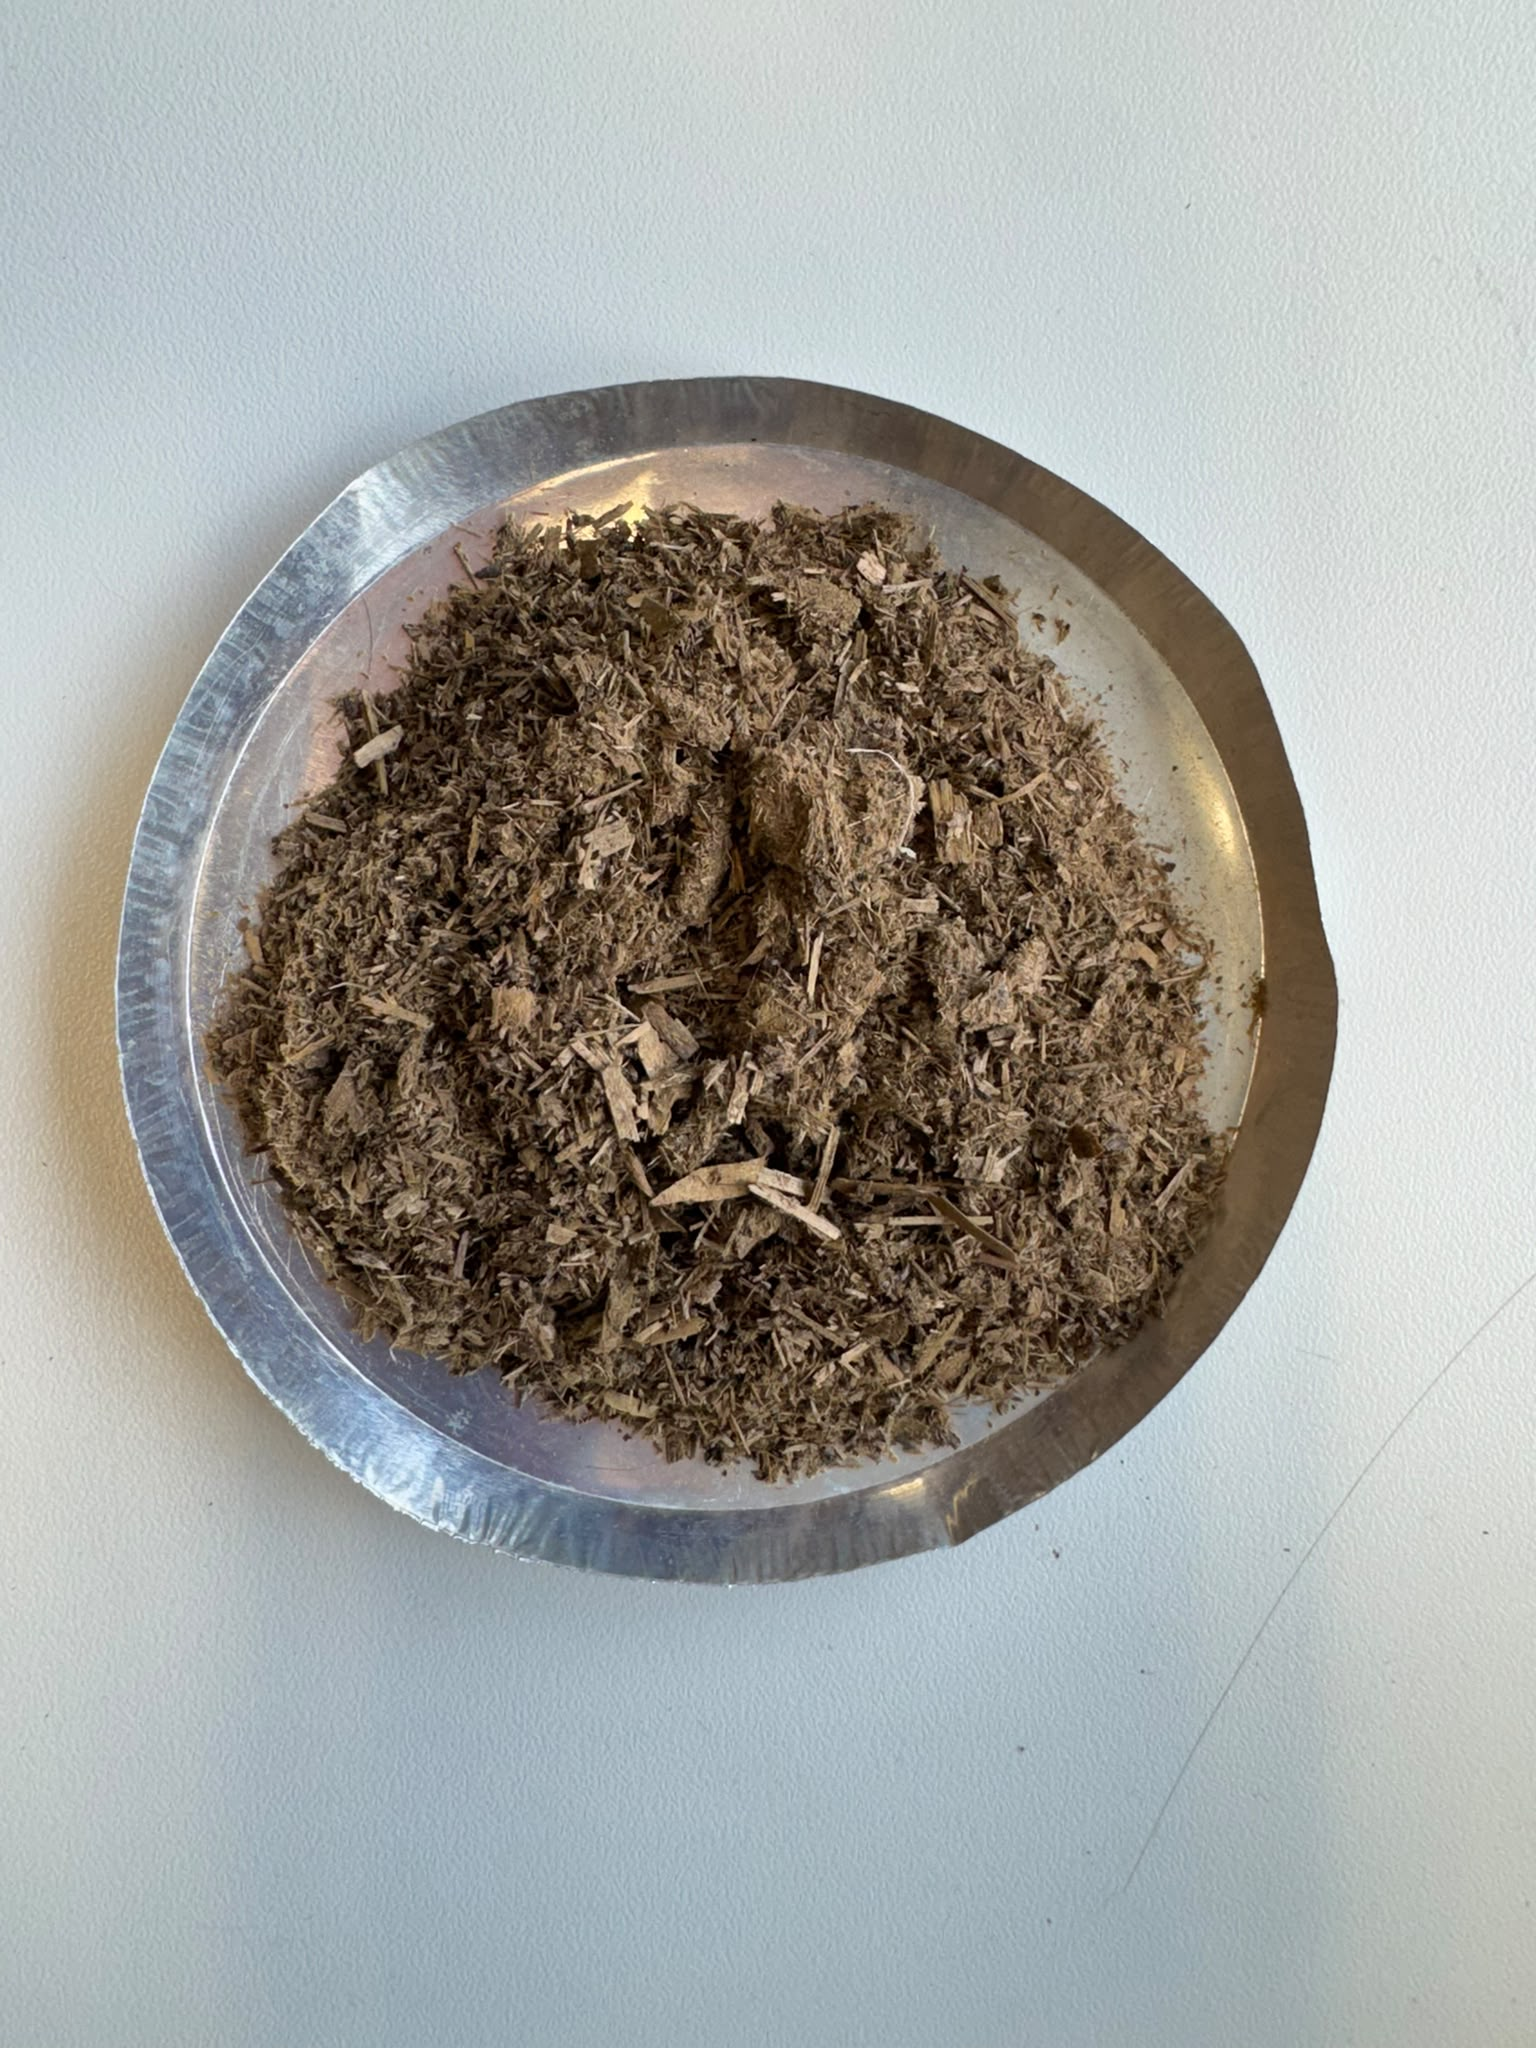
\includegraphics[angle=-90,origin=c]
            {Abbildungen/Algerian Digestate.jpeg}
        }
        \captionof{figure}{
            Algerian digestate obtained from the Centre de Développement
            des Energies Renouvelables (CDER) in Algiers, Algeria.
        }
        \label{fig:3.11}
    \end{minipage}
    \hfill
    \begin{minipage}[t]{0.49\linewidth}
        \centering
        \resizebox{\linewidth}{!}{%
            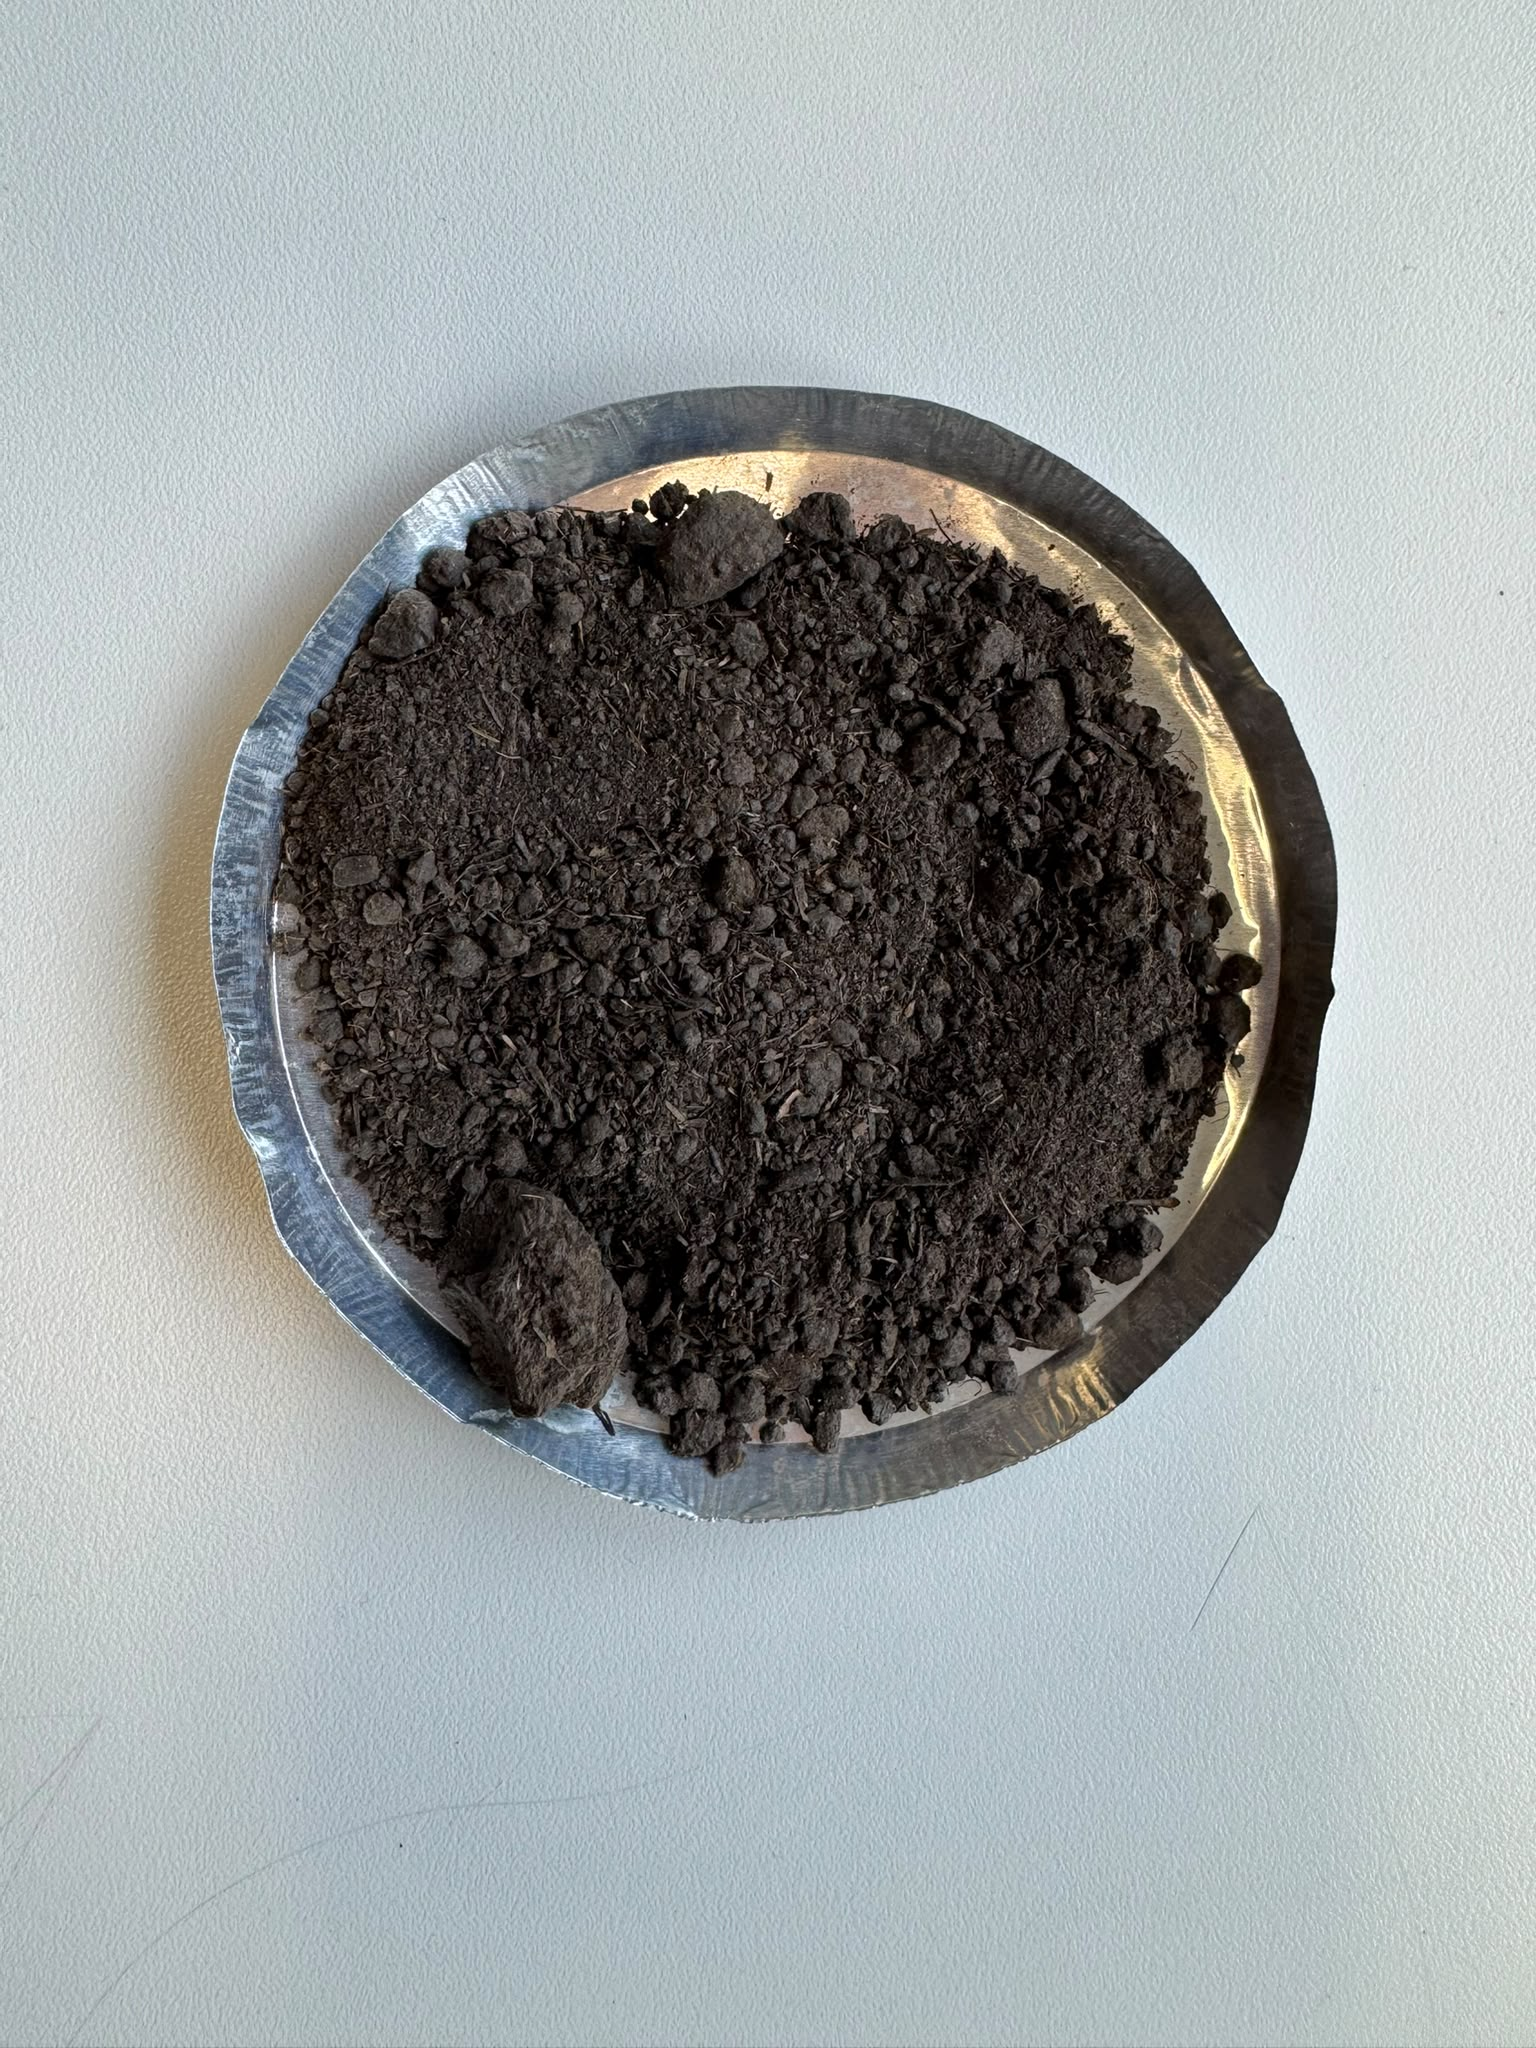
\includegraphics[angle=-90,origin=c]
            {Abbildungen/French Digestate.jpeg}
        }
        \captionof{figure}{
            French digestate obtained from the Centre National de la Recherche
            Scientifique (CNRS-ICARE) in Orléans, France.
        }
        \label{fig:3.12}
    \end{minipage}

\end{figure}

\vspace{0.3em}

The digestate was used in its as-received state for the pyrolysis experiments. After pyrolysis, the resulting biochars were stored in a desiccator to prevent moisture uptake during subsequent storage and handling. A separate drying step using a moisture-analyzing device was applied to digestates and biochars prior to calorific value determination.

\vspace{0.3em}

The reagents and gasses employed in the activation and sulfurization steps were:
\begin{itemize}
    \item Deionized water ($H_2O$) - Activation agent
    \item Argon, $Ar$ with 99,999\% purity - Inert gas for purging prior to activation
    \item Iron(II) sulfide, $FeS$ - sulfide source for $H_2S$ generation
    \item Hydrochloric acid, H$Cl$ - acid reagent for $H_2S$ generation
\end{itemize}

\subsection{Biochar Production via Pyrolysis}
\setresponsible{Surya Salim}
\label{biocharproduction}

Biochar was produced in the laboratory for thermochemical processes in Department 1: Engineering—Energy and Information at the Berlin University of Applied Sciences (HTW Berlin). Biochar was produced from both digestates by slow pyrolysis in an electrically heated laboratory-scale oven. The setup consisted of a programmable temperature-controlled oven and a sealable pyrolysis reactor, as shown in Figure~\ref{fig:3.2.1}. The required heating temperature and duration for the pyrolysis process were set and regulated using the button located right below the chamber. Inside the oven, white refractory ceramic insulation material is used to withstand high temperatures and reduce heat transfer to the outside, ensuring an uniform temperature inside the heating chamber. 

\begin{figure}[H]
    \centering
    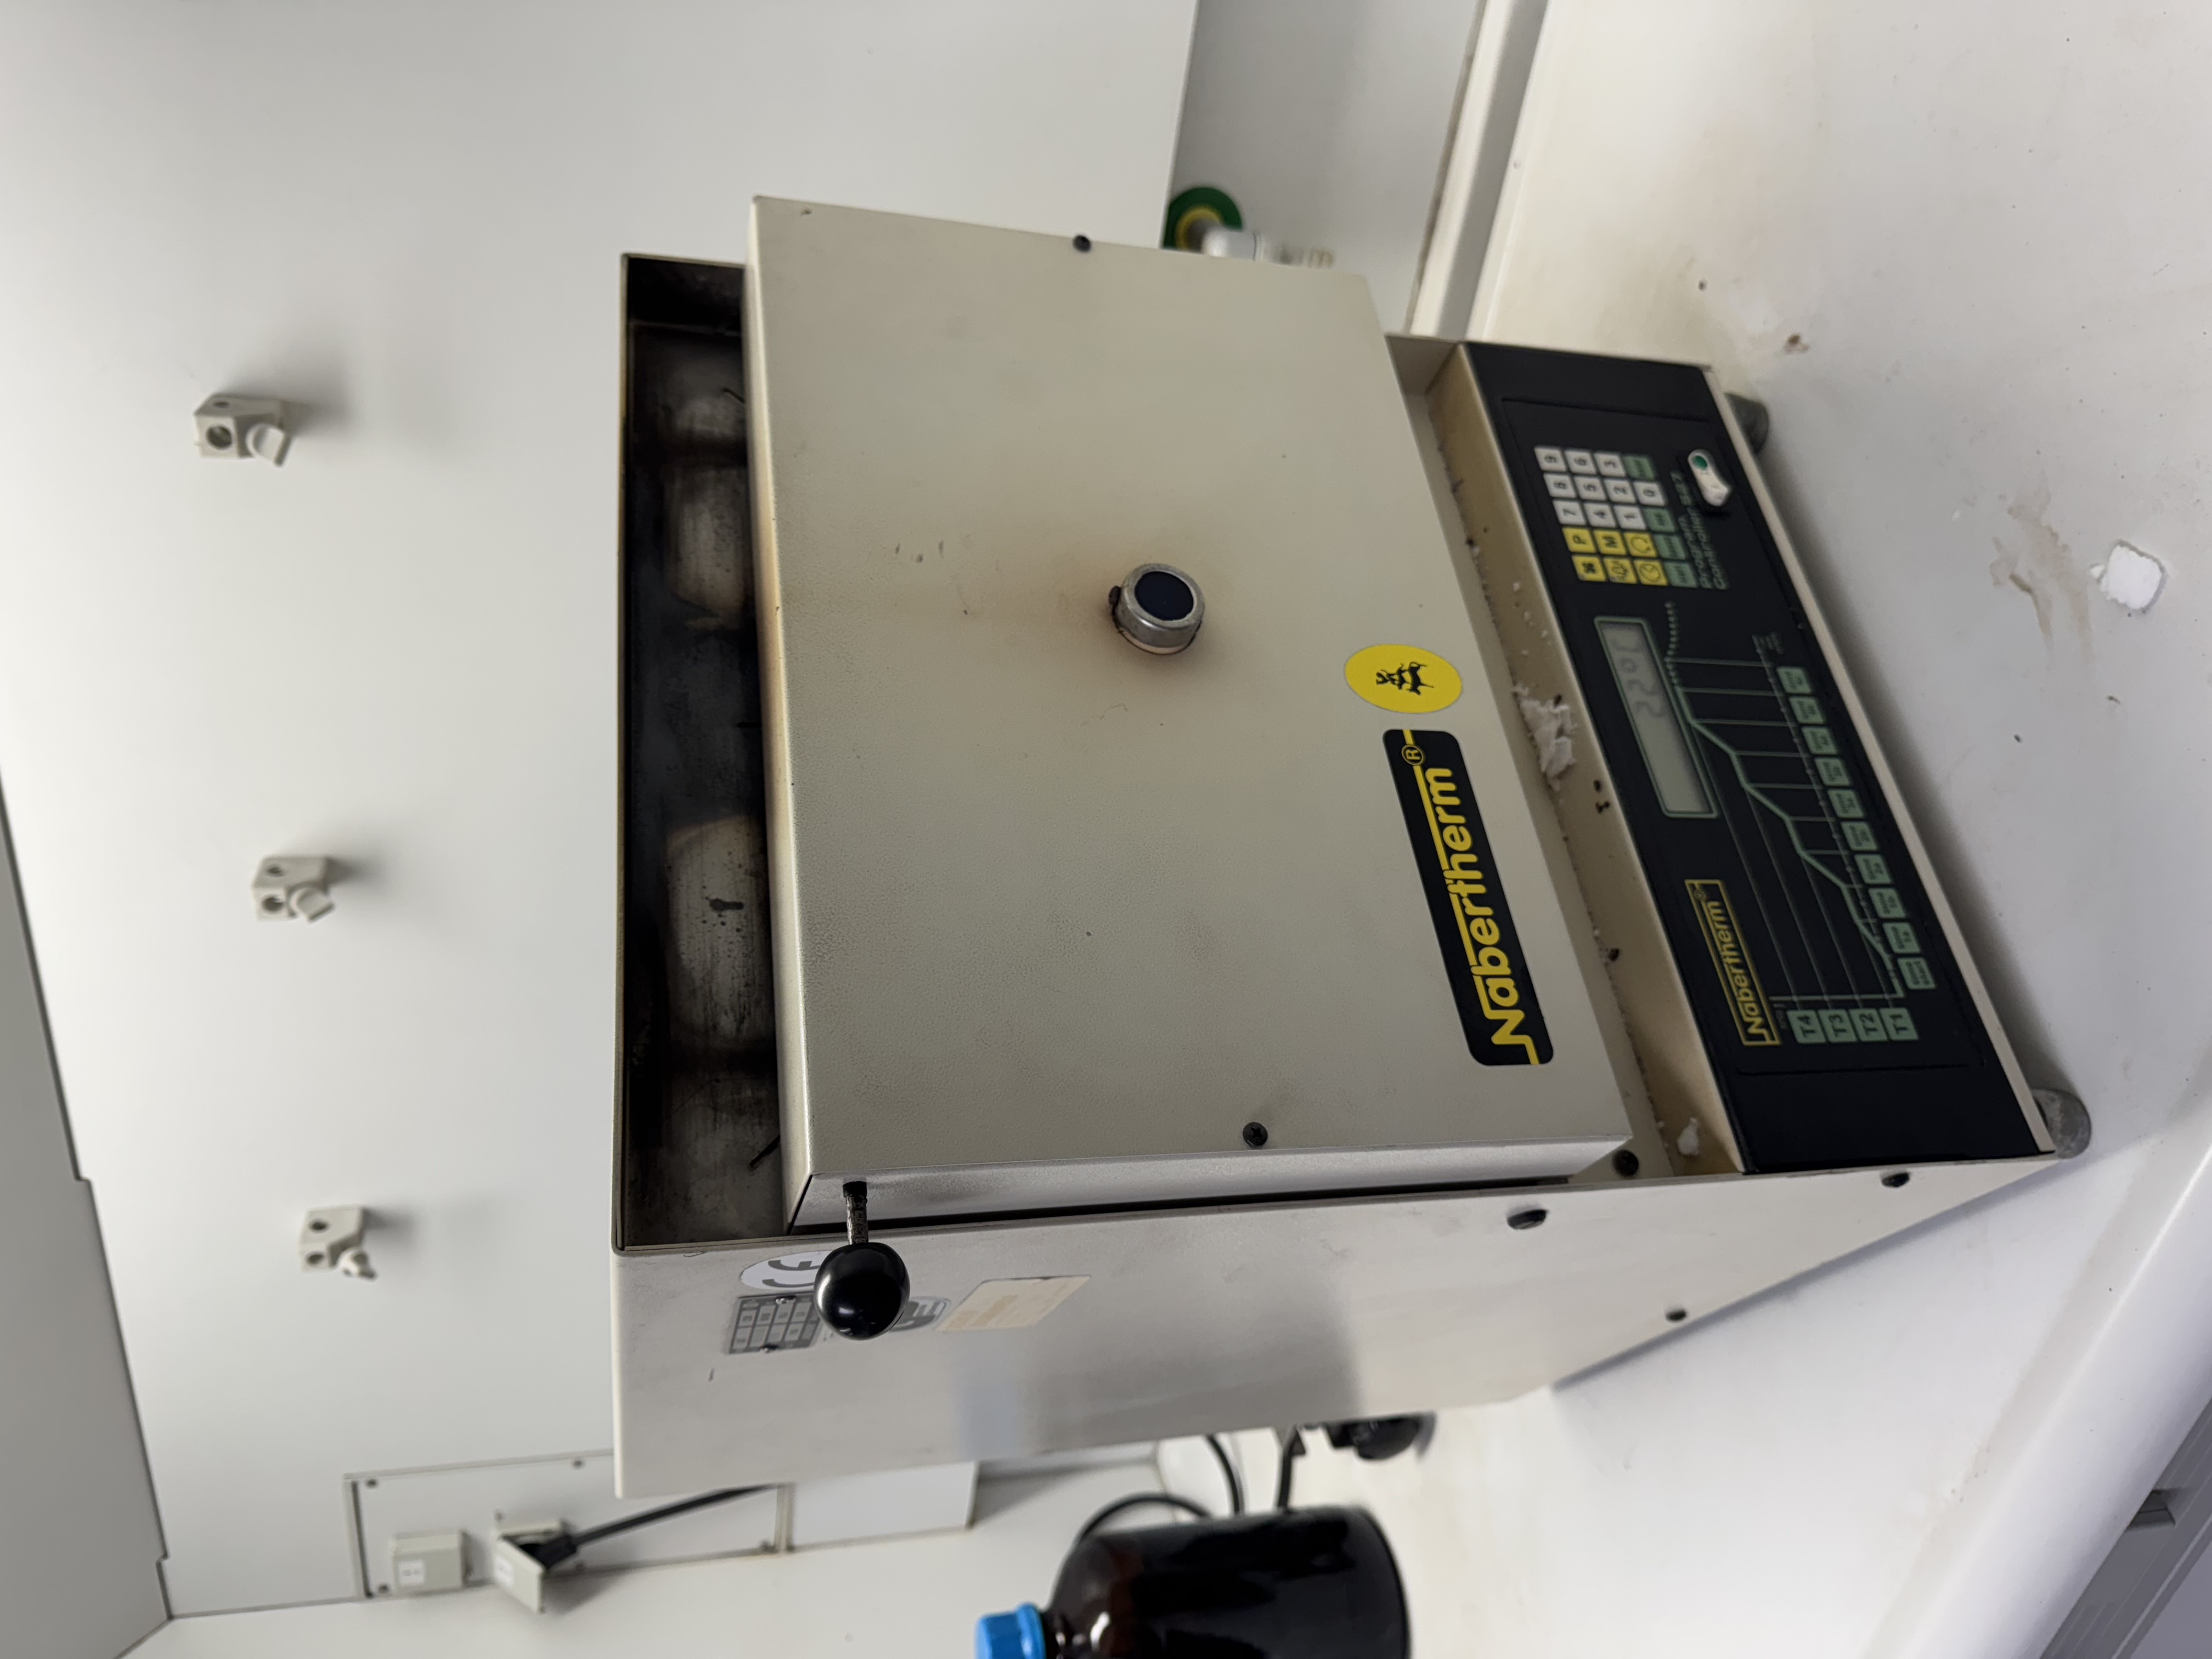
\includegraphics[width=0.8\linewidth, angle=-90]{Abbildungen/Pyrolissi oven.jpeg}
    \caption{Experimental setup for slow pyrolysis}
    \label{fig:3.2.1}
\end{figure}

\vspace{0.3em}

Prior to each run, the reactor was thoroughly cleaned to ensure consistency between experiments, and the gas outlet pipe was inspected to prevent blockages during operation. Due to the limited quantity of the primary substrate (Slaughterhouse digestate, France), pyrolysis was carried out using ceramic crucibles Figure~\ref{fig:3.2.2}, placed inside the reactor rather than by filling the reactor volume directly, as illustrated in Figure~\ref{fig:3.2.3} and \ref{fig:3.2.4} .

\begin{figure}[H]
    \centering
    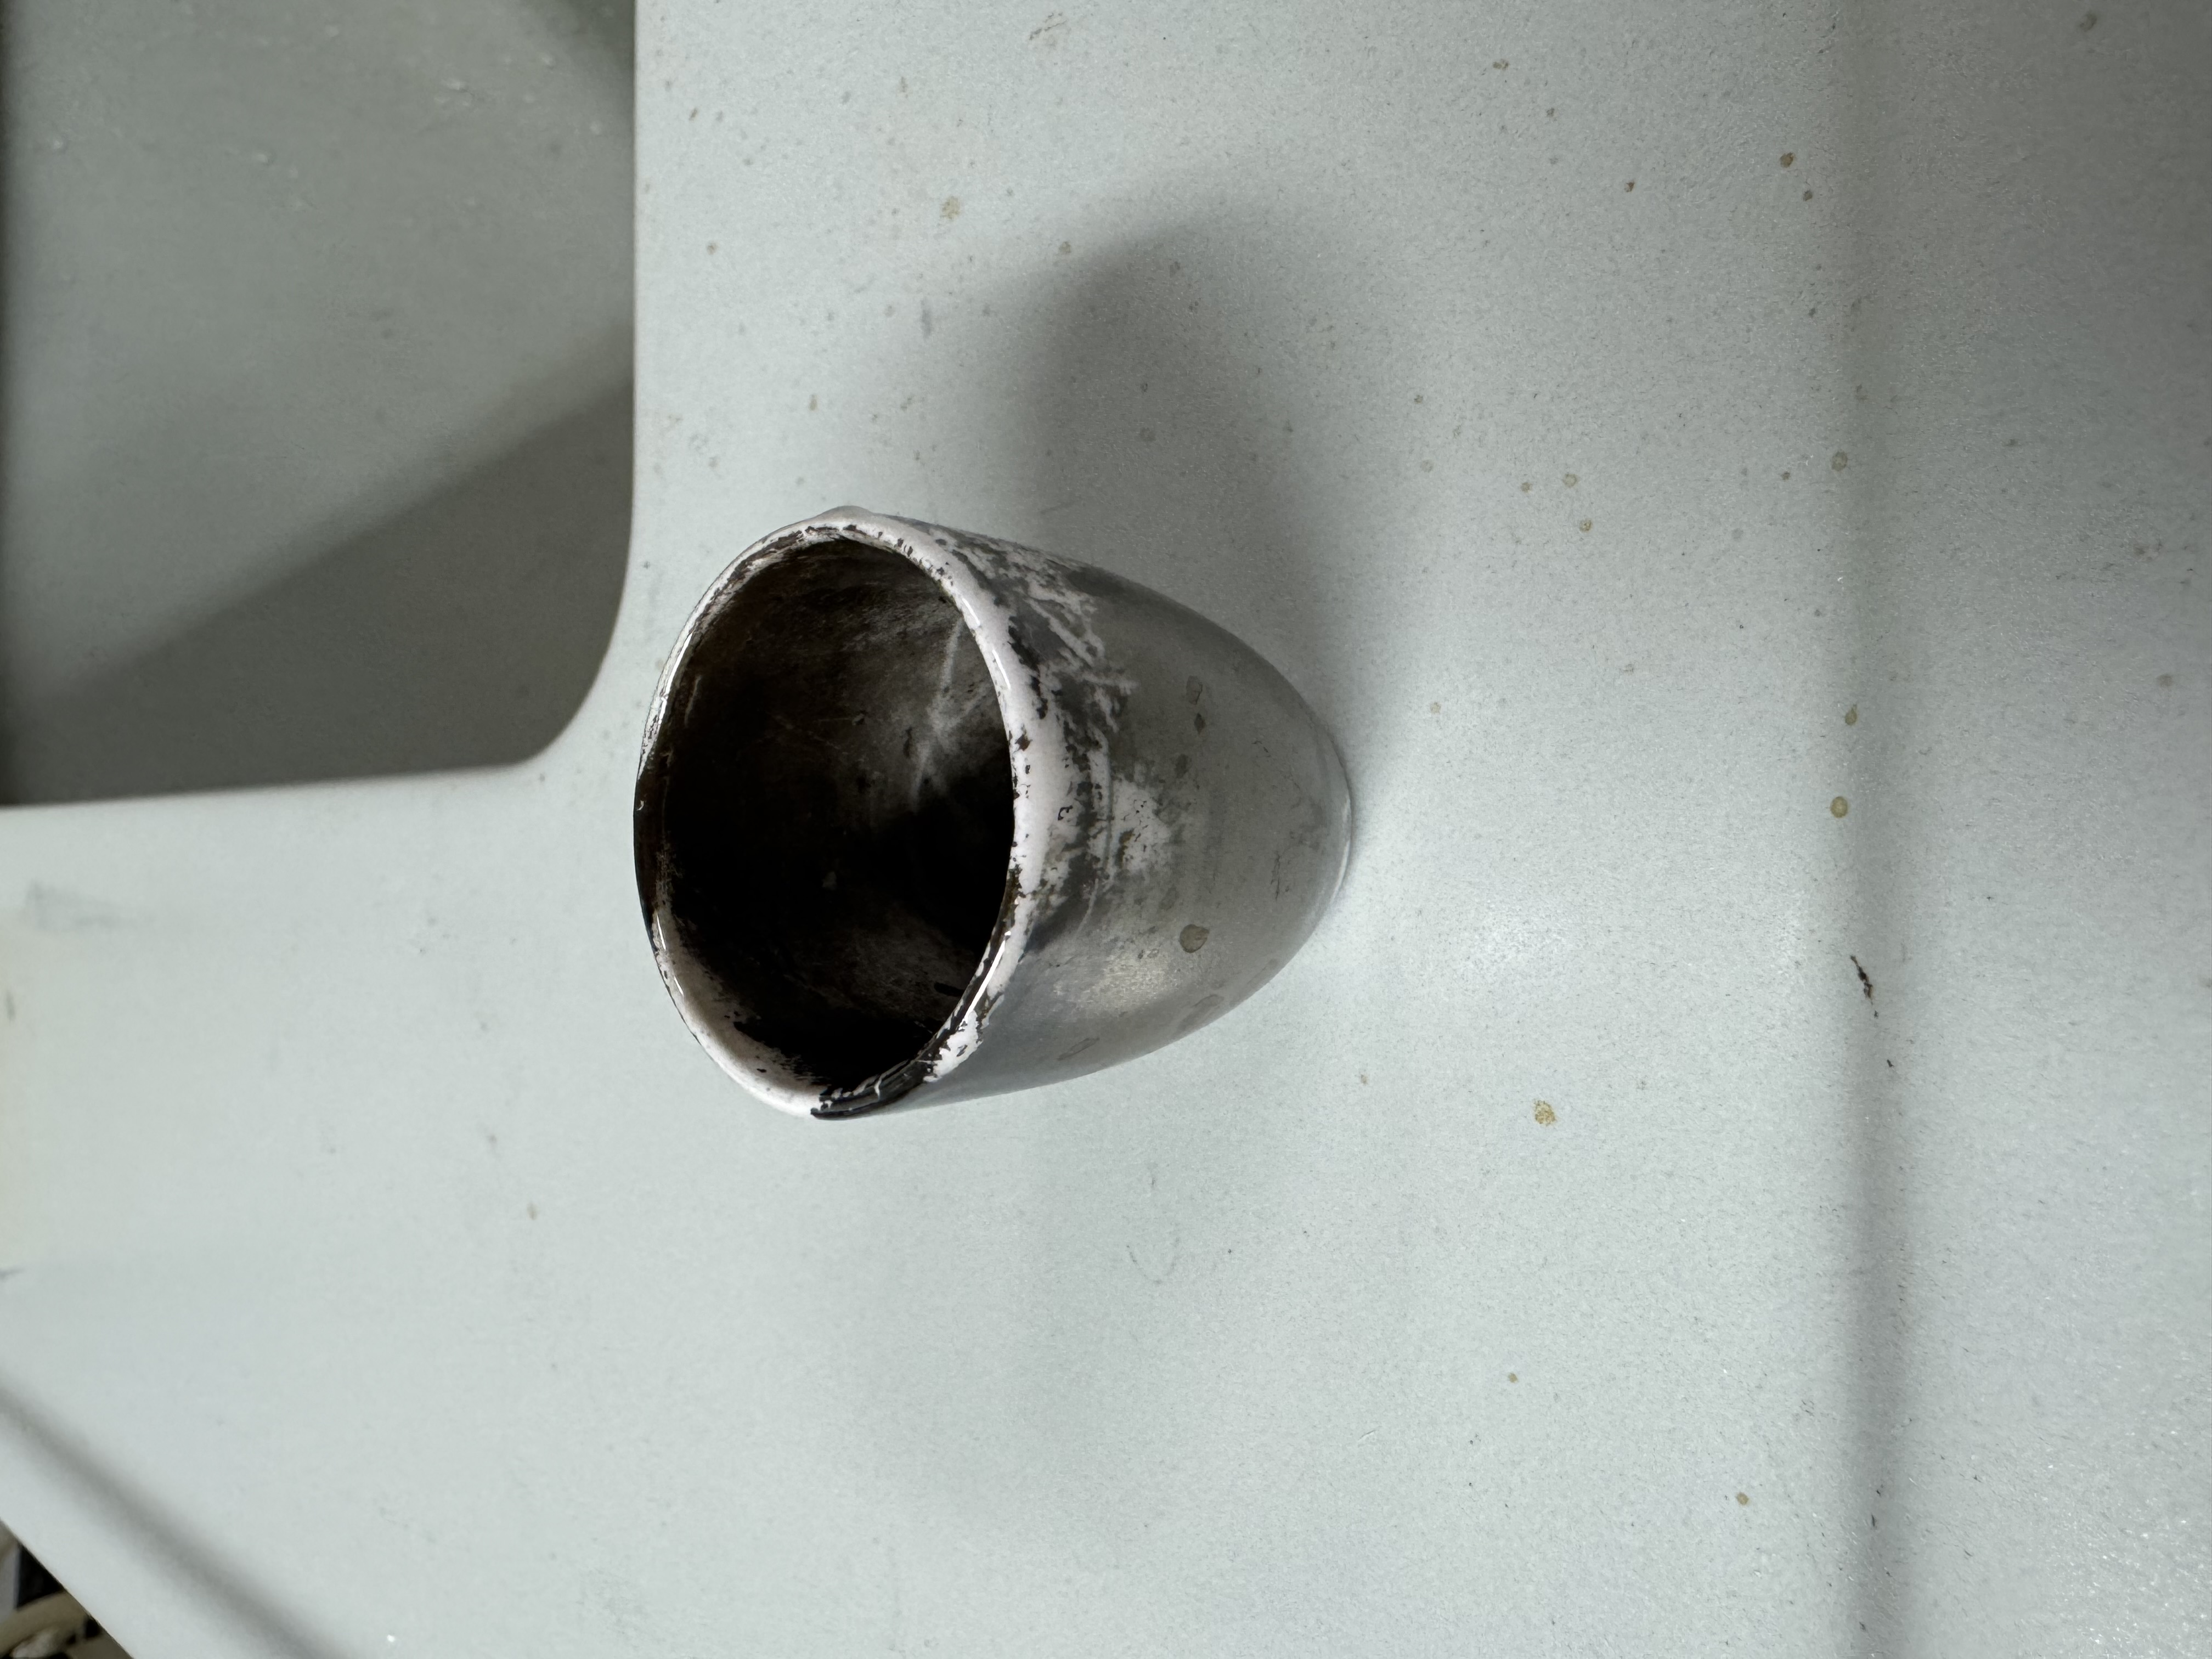
\includegraphics[width=0.7\linewidth, angle=-90]{Abbildungen/Crucible.jpeg}
    \caption{Ceramic crucible}
    \label{fig:3.2.2}
\end{figure}

\begin{figure}[H]
    \centering
    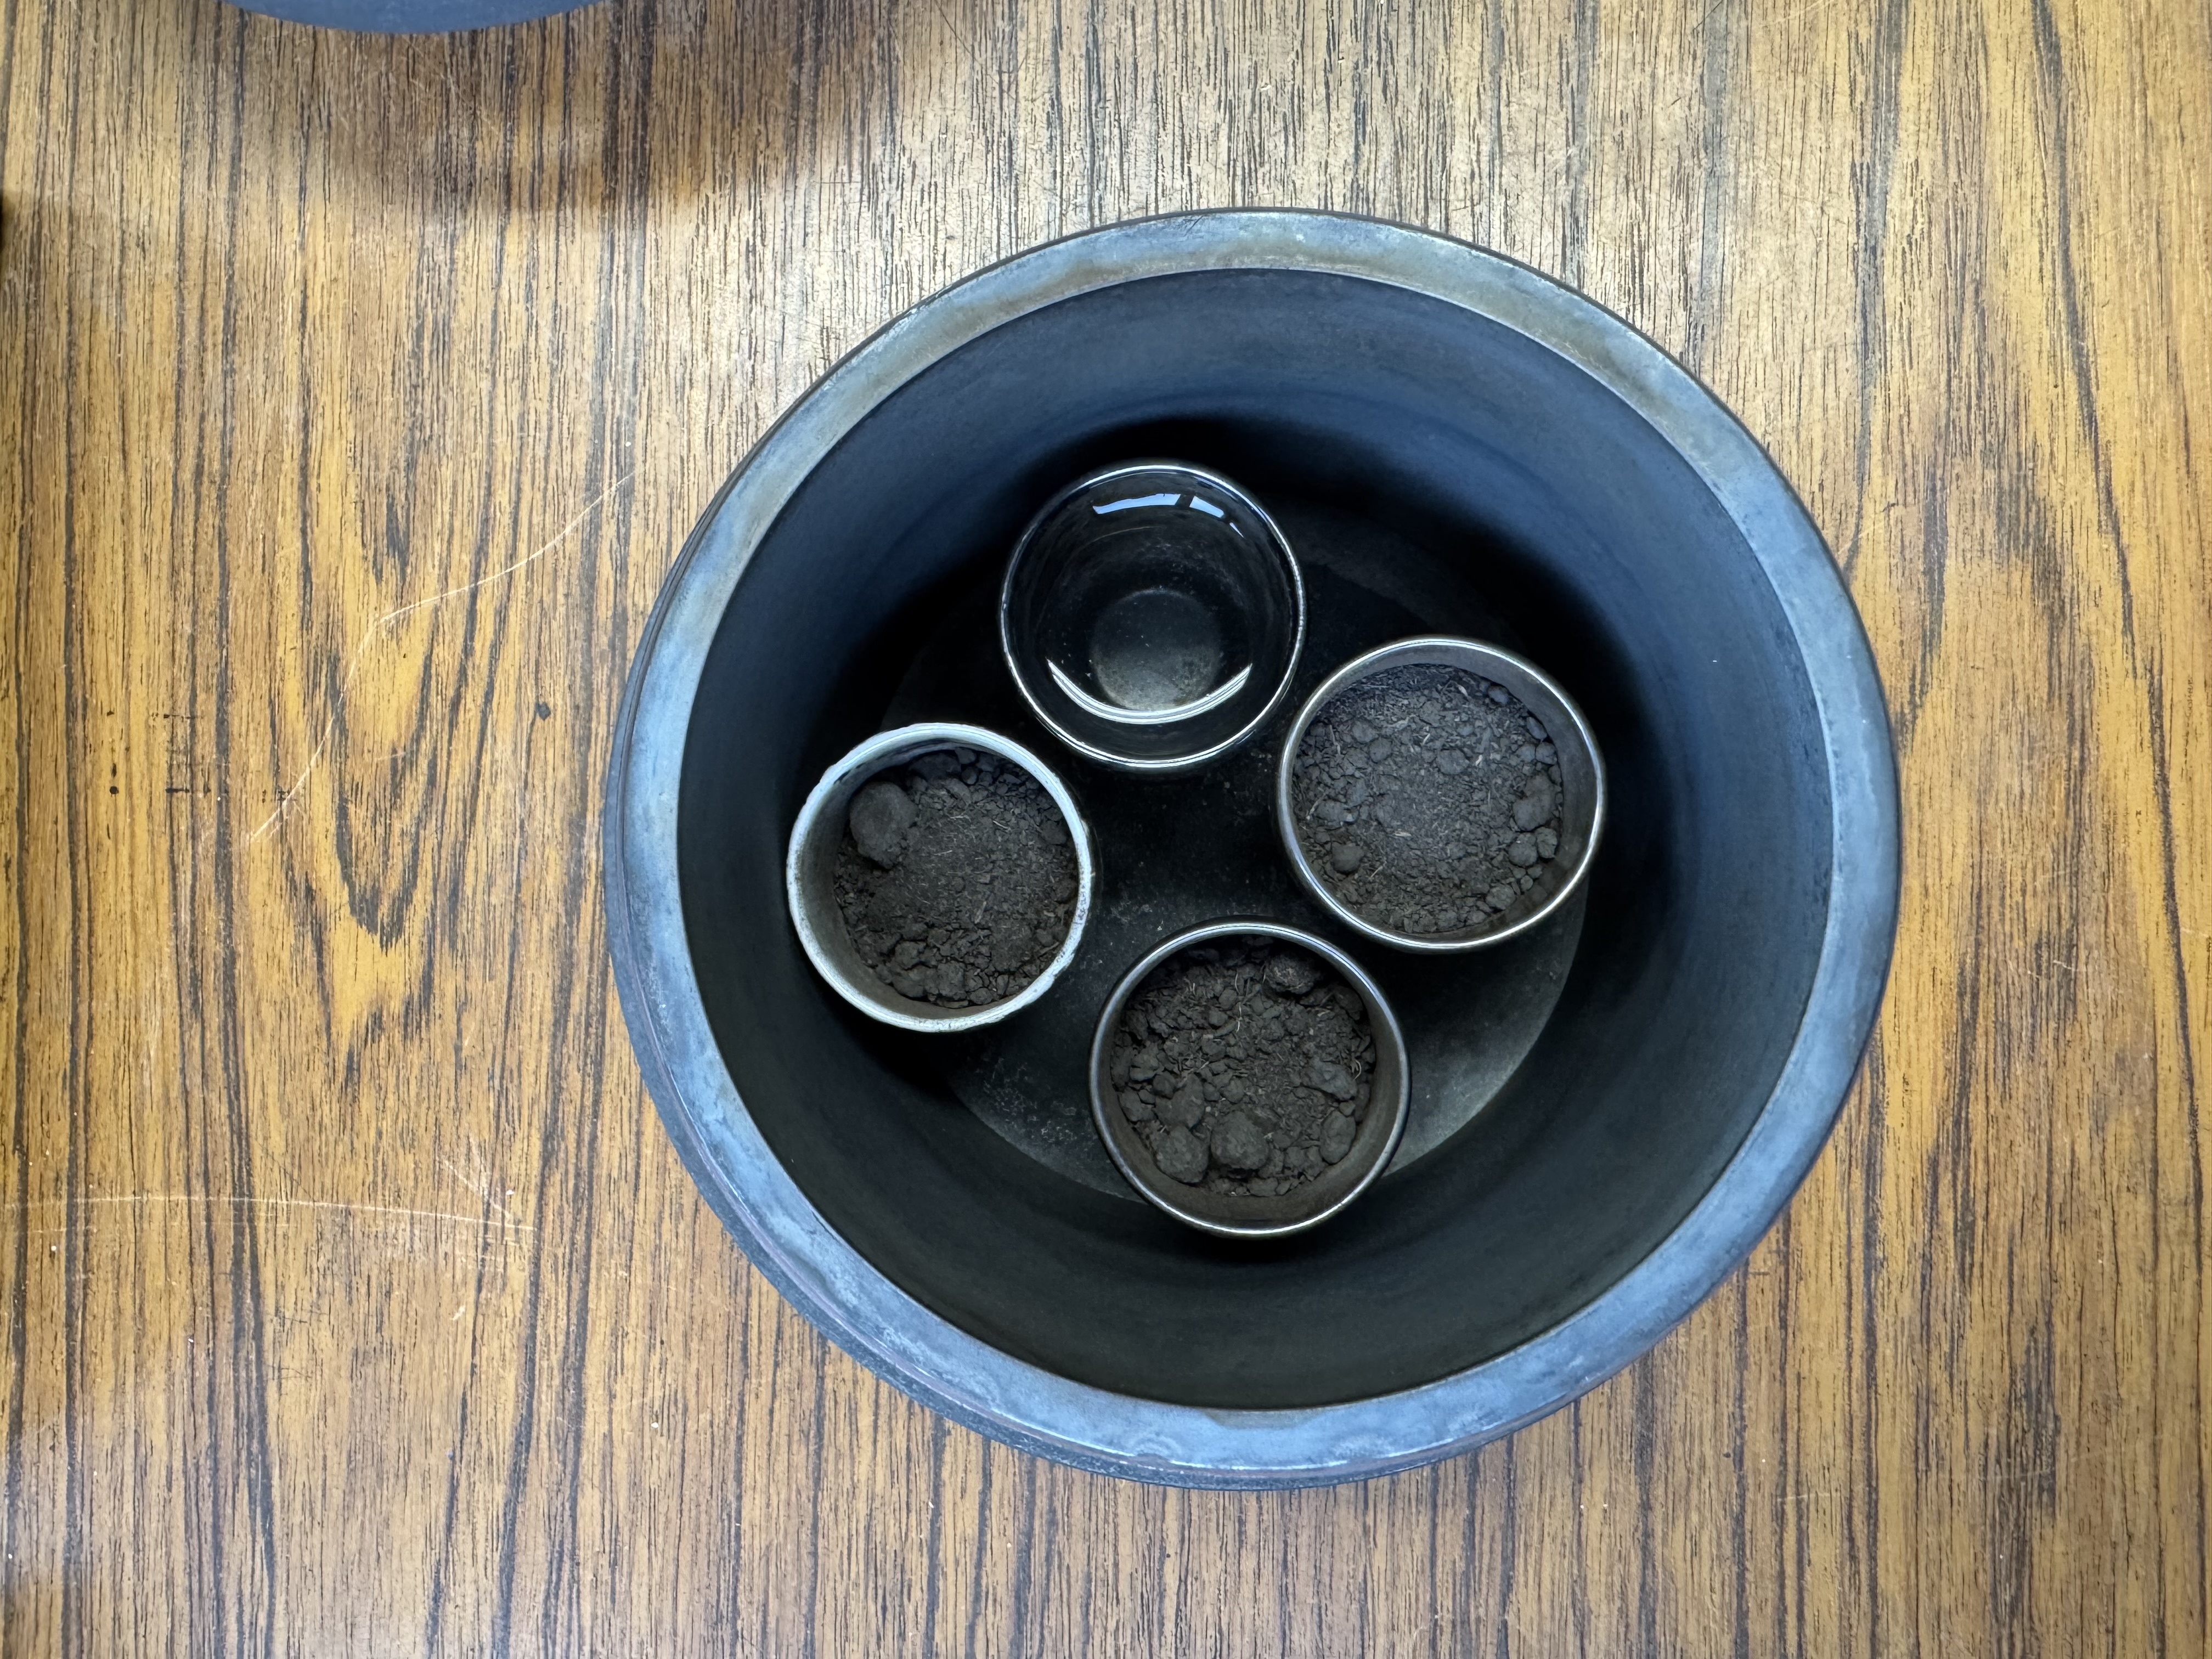
\includegraphics[width=0.8\linewidth]{Abbildungen/IMG_0003 (1).jpeg}
    \caption{The ceramic crucibles filled with biomass and water inside the reactor}
    \label{fig:3.2.3}
\end{figure}

\begin{figure}[H]
    \centering
    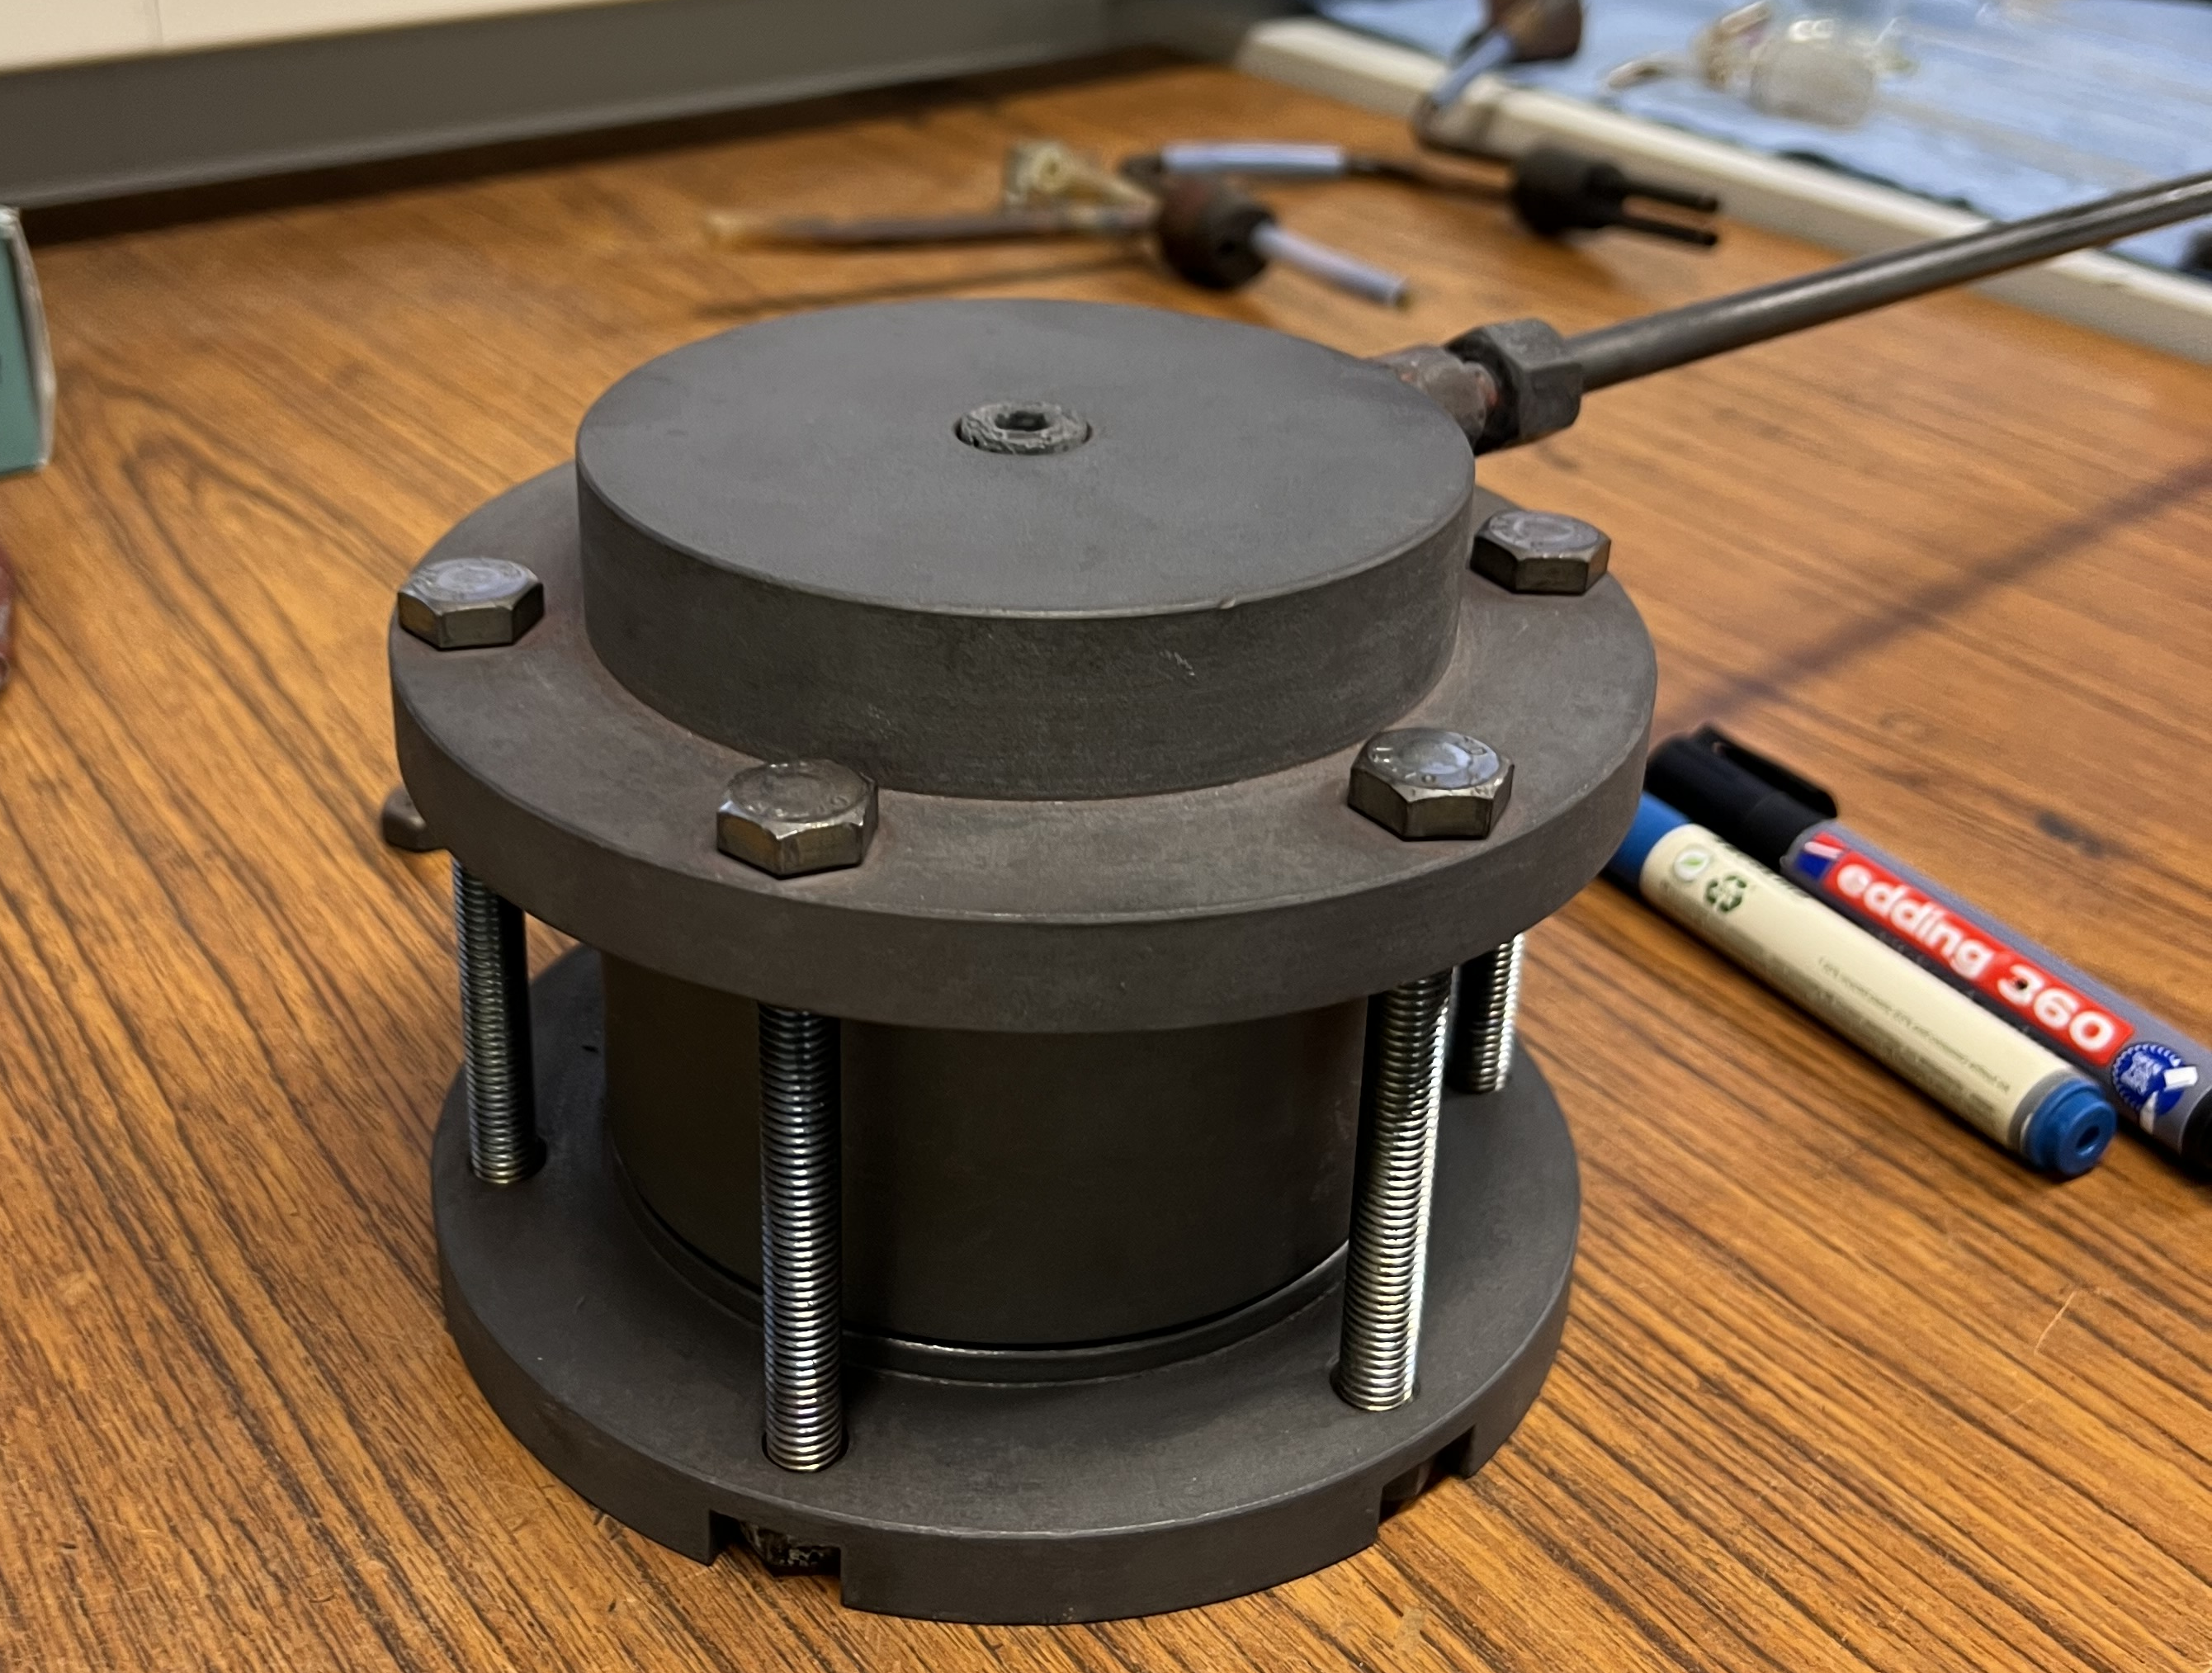
\includegraphics[width=0.8\linewidth]{Abbildungen/Cut-reactor.png}
    \caption{The reactor}
    \label{fig:3.2.4}
\end{figure}

\vspace{0.3em}

For each run, a known mass of digestate (recorded before pyrolysis) was loaded into the crucibles, and an additional crucible containing a defined mass of water was placed alongside the sample crucibles. The water generated water vapor during heating, which helped maintain an oxygen-poor atmosphere within the reactor. 

\vspace{0.8em}

The reactor was first sealed with 6 screws, then placed inside the oven, and heated according to the following programmed conditions:
\begin{itemize}
    \item Heating rate : 10 °C min$^{-1}$
    \item Target temperatures : 400 °C, 500 °C, or 600 °C
    \item Residence time at target temperatures: 1 h
\end{itemize}

Three pyrolysis temperatures were investigated to study the influence of pyrolysis temperature on biochar yield and properties, as discussed in \S~\ref{Influence pyrolysis condition}. After the residence time, the oven was switched off and the reactor was allowed to cool down to relative lower temperature before opening, in order to avoid oxidation of the freshly produced biochar by atmospheric oxygen.

Only the solid product (biochar) was collected and quantified in this study. The condensable bio-oil and non-condensable gas fractions were neither quantified nor characterized. The biochar yield Y was calculated as:
\begin{equation}
    Y = \frac{m_{Biochar}}{m_{Digestate}} \times 100 \%
    \label{eq:biochar yield}
\end{equation}
where $m_{Digestate}$ is the initial mass of digestate loaded into the reactor and $m_{Biochar}$ is the mass of the solid product recovered after pyrolysis. The collected biochars were transferred to plastic containers with name labels on them and stored until further processing in the activation step.

\subsection{\texorpdfstring{H$_2$O}{H2O}-Activation}
\setresponsible{Surya Salim}
\label{subsec:methods-activation}

To develop the porous structure of the biochar produced in \S~\ref{biocharproduction}, a steam activation step was carried out in a separate setup consisting of a horizontal tube furnace (Carbolite) and a reaction tube placed coaxially inside the furnace, as shown in Figures~\ref{fig:3.3.1} and~\ref{fig:3.3.2}. The reaction tube is sealed at both ends by valve-controlled fittings, allowing controlled gas flow during heat-up and full isolation of the reaction volume once the steam phase is initiated. The H$_2$O activation was carried out in the chemistry lab of Department 1: Engineering—Energy and Information, in Building F at the Berlin University of Applied Sciences (HTW Berlin). The activation was carried out exclusively on the biochar produced from the French digestate. The French biochar was designated as the primary substrate for the activation, sulfur loading and characterization steps that follow.
\begin{figure}[ht!]
    \centering
    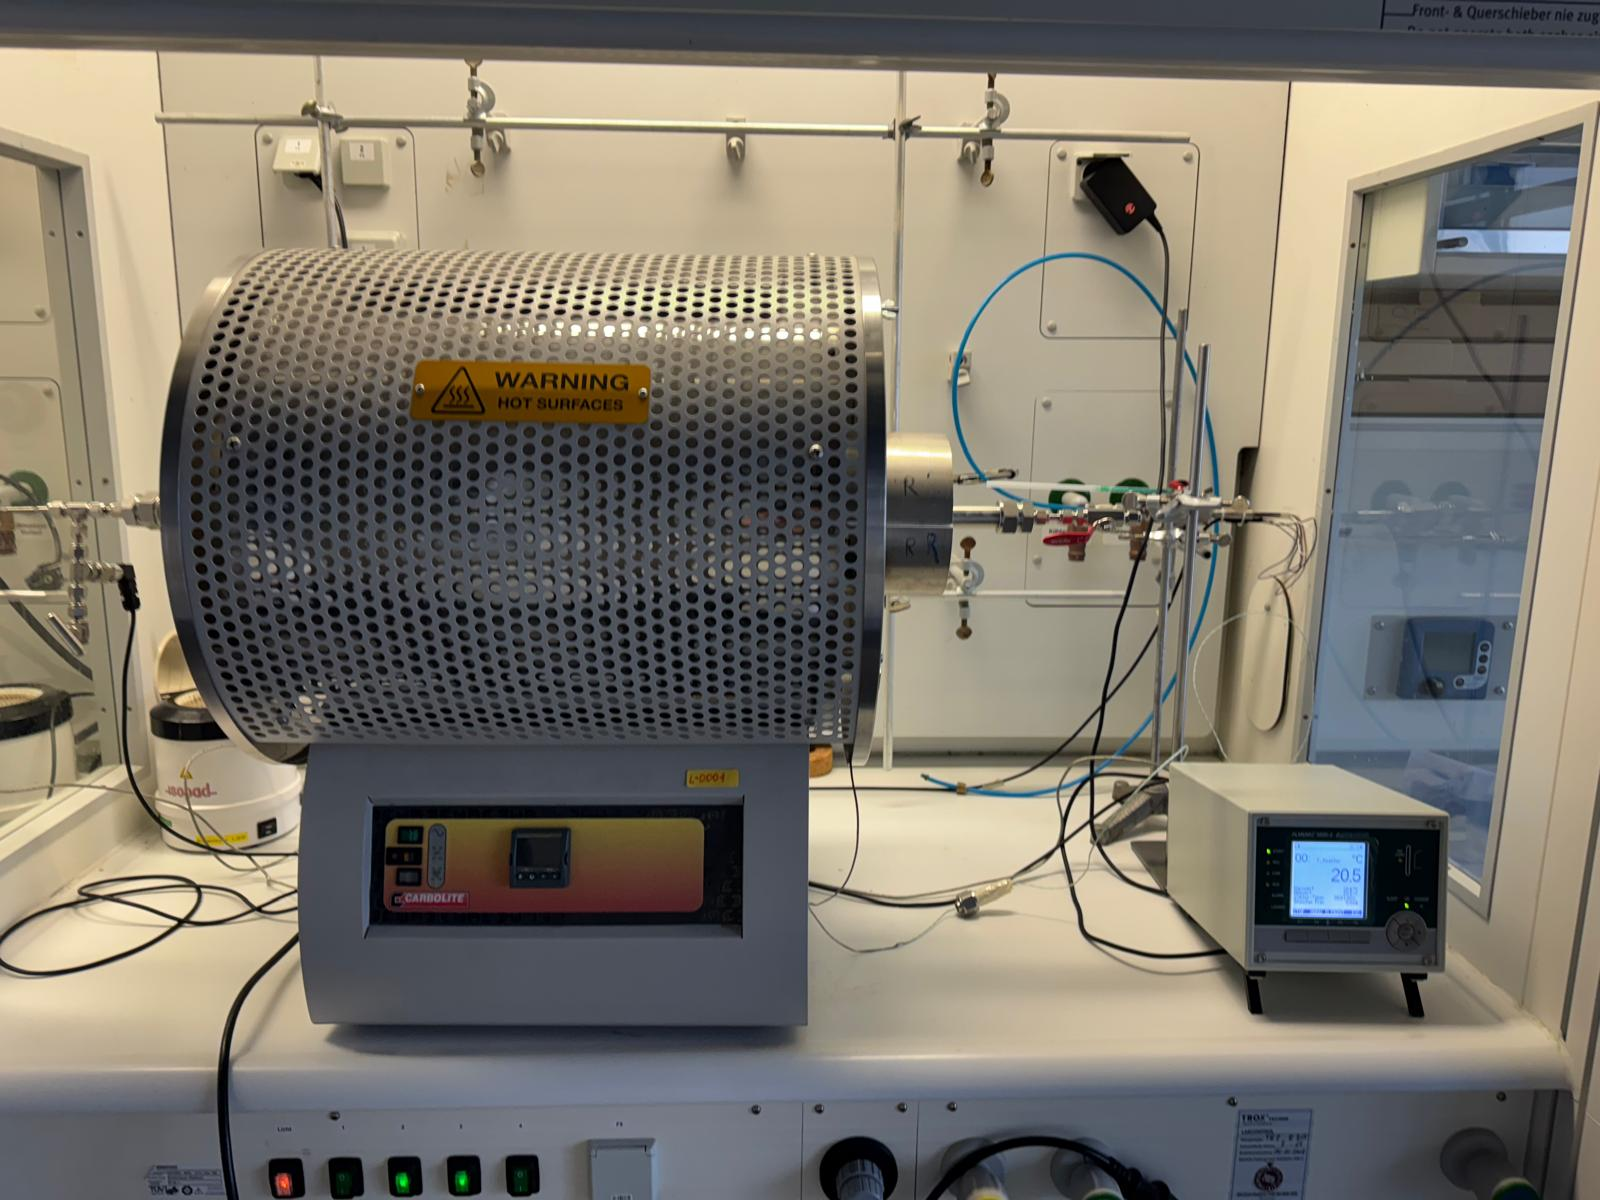
\includegraphics[width=0.8\linewidth]{Abbildungen/Aktivierungsetup.jpeg}
    \caption{Experimental setup for the steam activation of biochar, comprising the tube furnace, reactor tube and temperature controller.}
    \label{fig:3.3.1}
\end{figure}

\begin{figure}[ht!]
    \centering
    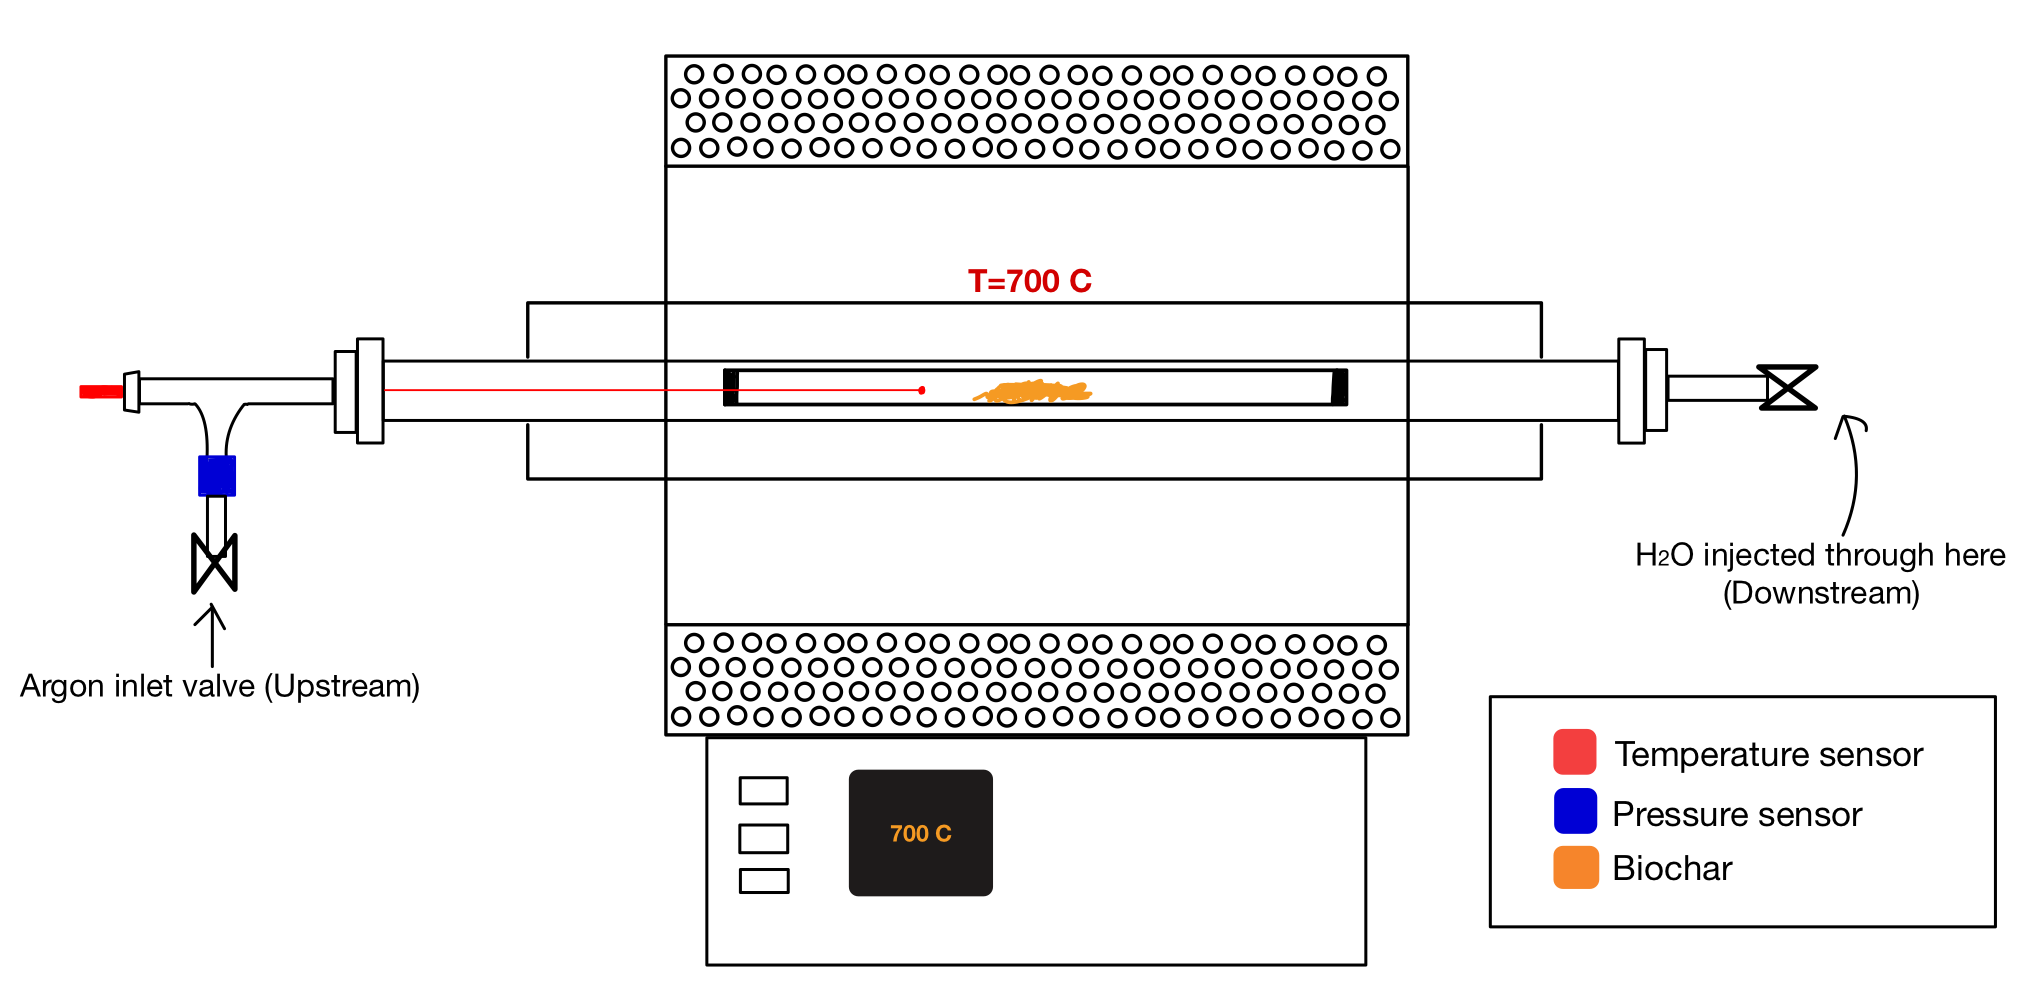
\includegraphics[width=0.8\linewidth]{Abbildungen/Aktivierungsovensketch.png}
    \caption{Schematic cross-section of the steam activation setup, showing the reactor tube within the tube furnace, with the biochar in the heated zone (T = 700 °C).}
    \label{fig:3.3.2}
\end{figure}

\vspace{0.8em}

The amount of water introduced per activation was selected to limit the mass loss of the biochar to below 10\%, in line with the burn-off control objective established in the project work. Although the underlying intent is to limit "carbon" loss, the experimentally accessible quantity in this work is the total mass loss of the biochar before and after activation. The two are equivalent only under the assumption that the steam-carbon reaction :
\begin{equation}
    C \, + H_2O \rightarrow CO \, + H_2
\end{equation}
is the sole mass-removing process. In practice, residual devolatilization of hydrogen- and oxygen-containing functional groups may also contribute to the measured mass loss.

\vspace{0.3em}

For this thesis, the biochar carbon content is assumed approximately 60\% based on preceding project work. Based on this number, a stoichiometric calculation for the respective reaction indicates that, at a uniform tube temperature of 700 °C, only about 0.09 g of water ($\approx$ 0.09 mL at STP) would theoretically be required to gasify 0.06 g of carbon. In practice, however, the temperature is not uniform across the entire tube volume; the central hot zone reaches the set point while the tube extremities remain considerably cooler, so that a non-negligible fraction of the injected water condenses on the cooler tube walls and is not available for reaction with the biochar. The maximum temperature was also set to 700 °C, since the pipe joint could not withstand temperatures exceeding 700 °C.

\vspace{0.3em}

To verify that the 10\% mass-loss target could be met under these non-ideal conditions, a comparative trial was carried out with two water doses applied to 1 g biochar from each pyrolysis temperature : 0.1 mL (close to the theoretical minimum) and 0.5 mL (a fivefold excess intended to compensate for steam losses to condensation). The resulting losses were essentially identical for the 500 °C  biochars (see table~\ref{tab:activation-full}). On the wet basis, both doses sat near or below 10\%, while moisture-corrected losses ran 10-22\%. 

\vspace{0.3em}

On this basis, the 0.5 mL of water per 1 g of biochar dose was adopted as the standard activation condition. All activated biochars used thereafter for the elemental and surface analyzes described in \S~\ref{sec: Analyticalmethods} were produced under this condition. The 0.1 mL dose was retained only as a comparative reference for the activation study. The same dose ratio was additionally checked at twice the scale. In runs 10--12 (Table~\ref{tab:activation-full}), 2\,g of biochar was activated with 1.0\,mL of water, and the
moisture-corrected mass losses followed the same descending order with pyrolysis temperature as
the corresponding 1\,g runs.

\subsubsection*{Activation procedure}
\begin{enumerate}
    \item \textbf{Inert purging and heat-up} \newline
    Argon was introduced from the upstream end (or left side of Figure \ref{fig:3.3.2}) of the tube and allowed to exit through the other end of the tube valve. The argon flow was kept deliberately low to maintain an inert atmosphere without blowing off the biochar. Simultaneously, the furnace was switched on and programmed to reach a set point of 700 °C at a heating rate of 10 K min$^{-1}$.
    \item \textbf{Transition to steam atmosphere} \newline
    Argon pushing was continued until the downstream end (or right side of Figure \ref{fig:3.3.2}) of the tube reached a temperature above 100 °C. This ensures that injected liquid water would flash to vapor rather than condense at the injection point. At this point, before injection, the argon flow was stopped and both valves of the tube were closed.
    \item \textbf{Water injection and sealed activation} \newline
    A single dose of 0.5 mL of deionized water was manually injected through the downstream valve using a syringe. The downstream valve was closed immediately after injection, isolating the reaction tube from the surrounding atmosphere. Under these closed-tube conditions, the injected water flashed to steam in the hot central region and reacted with the biochar over the activation period. The 1 h activation period was timed from the moment of water injection. Some condensation of steam in the cooler tube extremities is expected. Consequently, not all of the injected water vapor is assumed to participate in the steam-carbon reaction.
    \item \textbf{Cool-down} \newline
    After the 1 h hold, the furnace was switched off and the system was allowed to cool to ambient temperature overnight.

    After cooling, the activated biochar was recovered from the reactor tube and weighed. The activation mass loss was calculated on a wet basis as:
    \begin{equation}
        \Delta m_{active,wet}=\frac{m_{before}-m_{after,wet}}{m_{before}} \times 100\%
    \end{equation}
    Because water was introduced during activation by spraying, this initial post-activation mass still contained moisture that had to be separated from the actual mass change caused by activation. Residual moisture was determined gravimetrically using another halogen moisture analyzer (PCE-MA series, PCE Instruments GmbH, Germany) operating on the loss-on-drying (LOD) principle. The instrument heats the sample by means of halogen lamps and calculates moisture content from the mass difference before and after drying; a drying temperature of 190 °C was used. As the analyzer required a minimum sample mass to produce a stable reading, two inert metal rings (combined mass $m_{Nutrings}$=20.74 g) were placed in the sample pan together with each biochar sample to meet this threshold. The rings were first dried so they contributed no moisture of their own, meaning the entire water mass detected during drying originated from the biochar.
    
    Because the analyzer reports moisture as a fraction of the total mass in the chamber, the reported value $w_{dryer}$ refers to the combined mass of biochar and metal rings rather than to the biochar alone. To get the true biochar moisture content:
    \begin{equation}
        w_{bio}=\frac{w_{dryer}\times(m_{after,wet}+m_{Nutrings})}{m_{after,wet}}
    \end{equation}
where $m_{after,wet}$ is the post-activation mass of the biochar prior to drying. After this  the value of $m_{after,dry}$ could be known thus also the total mass loss both from activation and also from the moisture which can be described as :
\begin{equation}
    \Delta m_{loss}=\frac{m_{before}-m_{after,dry}}{m_{before}} \times 100\%
\end{equation}
    \begin{equation}
        \Delta m_{loss}=\frac{m_{before}-(m_{after,wet}(1-w_{bio}))}{m_{before}} \times 100\%
    \end{equation}
    where $m_{before}$ is the mass of biochar loaded into the tube and $m_{after,dry}$ is the post-activation mass after drying. The activated biochars were stored in a glass container until further use in the sulphurization step.
\end{enumerate}

\subsection{Sulfur Loading}
\label{subsec:methods-sulfur-loading}
\setresponsible{Regen Wijaya}

The sulfur loading was carried out in the same chemistry laboratory where the H$_2$O activation took place. The sulfur loading process is carried out exclusively for activated biochar produced from French digestates. The process was conducted in the same chemistry laboratory room, using a simple laboratory-scale setup that resembles the principal process of biogas desulfurization. The setup consists of a magnetic stirrer, a reaction flask equipped with a dropping funnel, glass tubes, and connector tube (Figure \ref{fig:Schwsetup}), all of which are placed in an enclosed chamber equipped with a suction function.

\vspace{0.3em}

\begin{figure}[ht!]
  \centering
  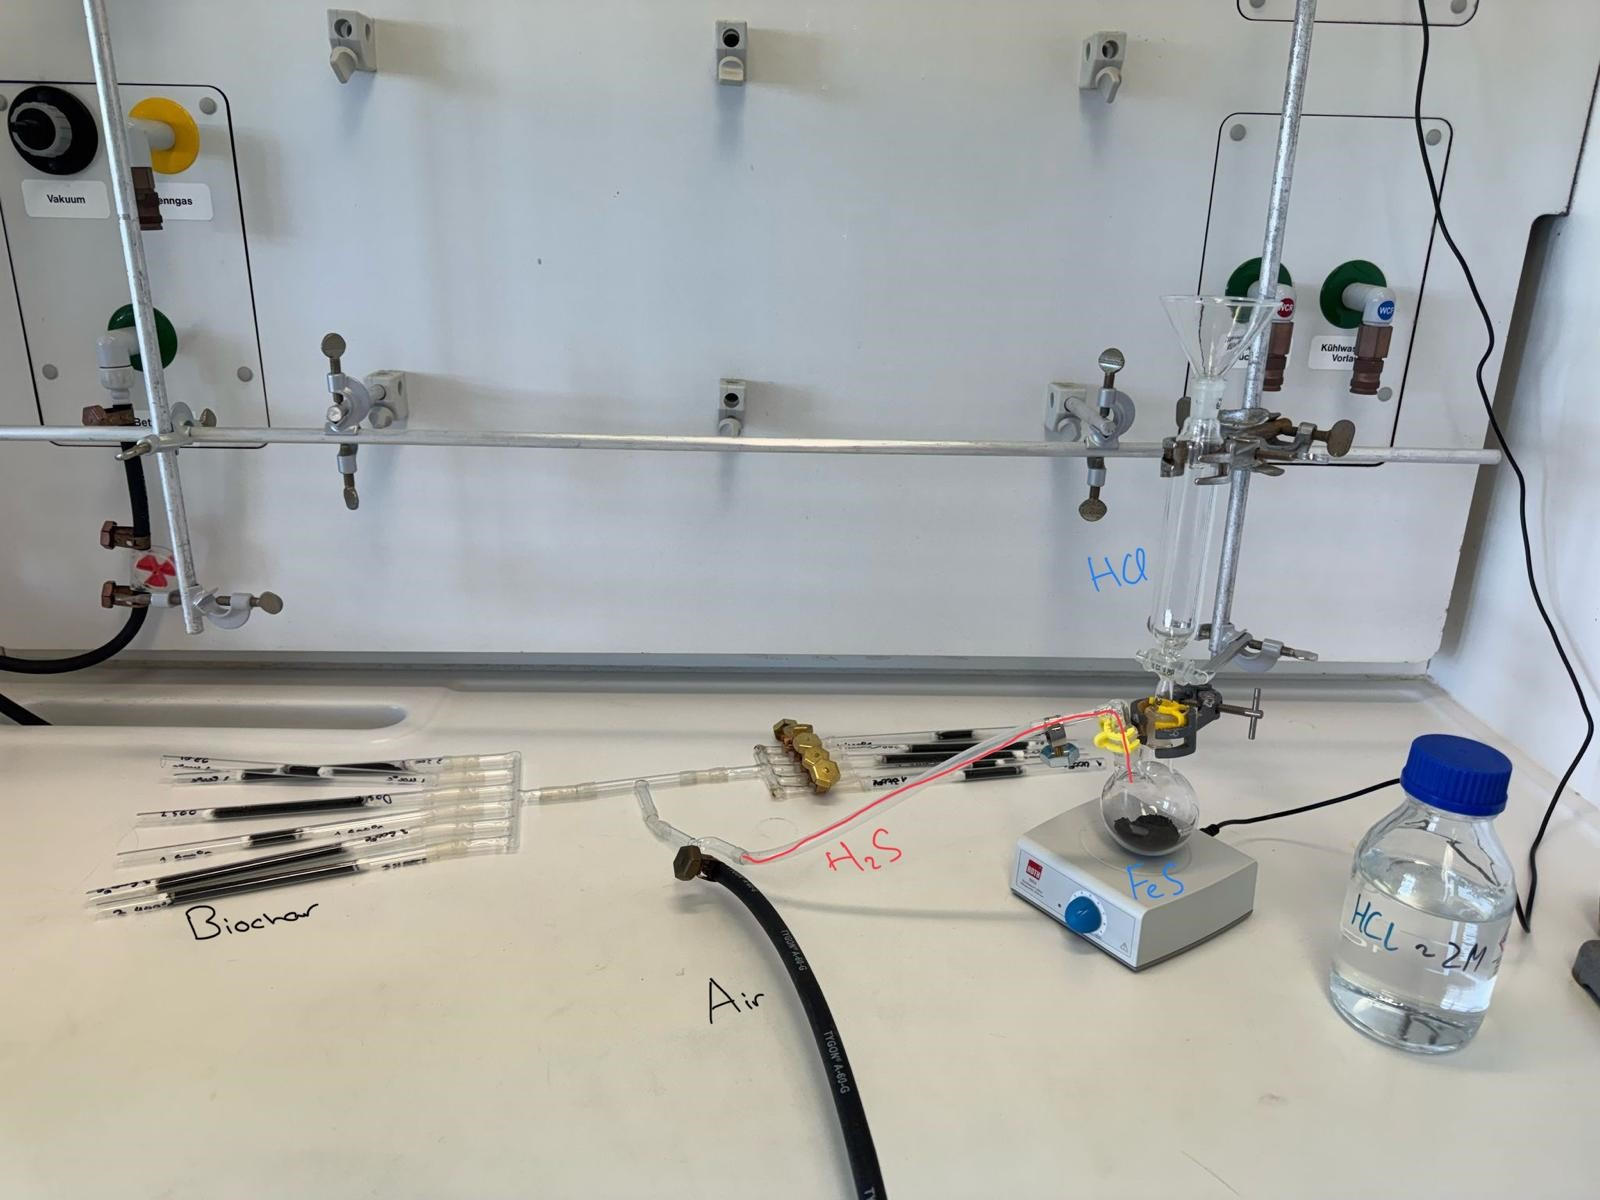
\includegraphics[width=0.8\linewidth]{Abbildungen/Schwefelbeladung Setup .jpg}
  \caption{The setup to load sulfur on the surface of biochar}
  \label{fig:Schwsetup}
\end{figure}

Firstly, the activated biochars were placed inside glass tubes that were open at both ends and plugged at both ends with cotton wool to keep the samples in place while allowing the gaseous flow of hydrogen sulfide to pass through without causing blockage. Each tube was connected to a Y-connector, which was linked to an air source and a reaction flask. 

\vspace{0.3em}

In the reaction flask, pulverized iron sulfide was placed and reacted gradually with droplets of hydrochloric acid from the funnel until the formation and release of hydrogen sulfide gas occurred, which can be characterized by the presence of continuous bubbling in the solution. The generated gaseous hydrogen sulfide was then directed to a Y-connector, where the $H_2S$ stream was introduced to the air stream. The resulting gaseous mixture then flowed through the activated biochars via each glass tube, where partial oxidation of H$_2$S to elemental sulfur was intended to occur on the biochar surface. The whole process lasted for approximately 30 minutes, allowing as much sulfur as possible to be absorbed on the surface of the biochar. Once the entire process was complete, the experimental setup was left undisturbed until the next day. The biochars were then dried and weighed.

\vspace{0.3em}

The sulfur adsorption capacity is represented by the quantity of sulfur adsorbed on the surface of biochar. It is evaluated gravimetrically by dividing the mass increase, which is the difference between the mass before and after the sulfur loading and drying process, by the initial mass of the biochar. It is then defined in milligrams per gram of biochar, as shown in Equation~\ref{Equation sulfur loading}.

\begin{equation}
q_s = \frac{m_{\mathrm{after,s}} - m_{\mathrm{before,s}}}{m_{\mathrm{before,s}}} \times 1000
\label{Equation sulfur loading}
\end{equation}

\subsection{Analytical Methods}
\label{sec: Analyticalmethods}
The analytical methods described in this section were applied to the raw digestate as well as to the biochars obtained after pyrolysis, $H_2O$ activation, and sulfurization, in order to evaluate the effect of each processing step on the resulting material properties.


\subsubsection{Calorific Value Determination (Bomb Calorimetry)}
\label{subsubsec:methods-calorimetry}
The higher heating value (HHV) of the raw digestate and the biochars was determined using an isoperibolic bomb calorimeter (IKA C 200, IKA-Werke GmbH \& Co. KG; Figure~\ref{fig:bombcalori}) following the principle described in \S~\ref{subsubsec:HHV}. The instrument was calibrated at the beginning of each measurement campaign using certified benzoic acid pellets, which served as the reference material for determining the effective heat capacity $\varepsilon$ of the calorimeter system.

\begin{figure}[htbp]
  \centering
  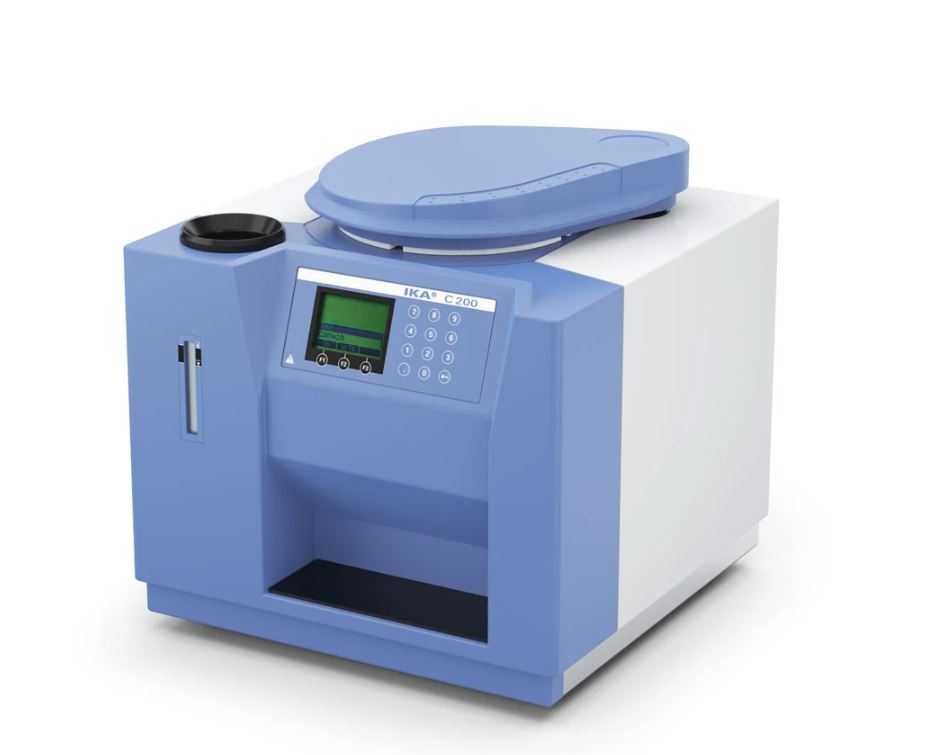
\includegraphics[width=0.88\linewidth]{Abbildungen/Kalorimeter.JPG}
  \caption{IKA calorimeter C 200}
  \label{fig:bombcalori}
\end{figure}

\vspace{0.3em}

Prior to each measurement, biochars were dried to remove residual moisture using a halogen moisture analyzer (PCE-MB 210C, Figure~\ref{fig:moisture_analyzer}) operated at 100°C until constant mass was reached, with the device evaluating dryness via a switch-off criterion of 10 s without further mass change. The dried biochars were transferred to a desiccator and kept there until measurement to prevent the re-uptake of atmospheric moisture. The moisture content displayed by the device was used solely as a process control to confirm that the biochar had reached a dry state and was not to be reported as an independent result.

\begin{figure}[H]
    \centering
    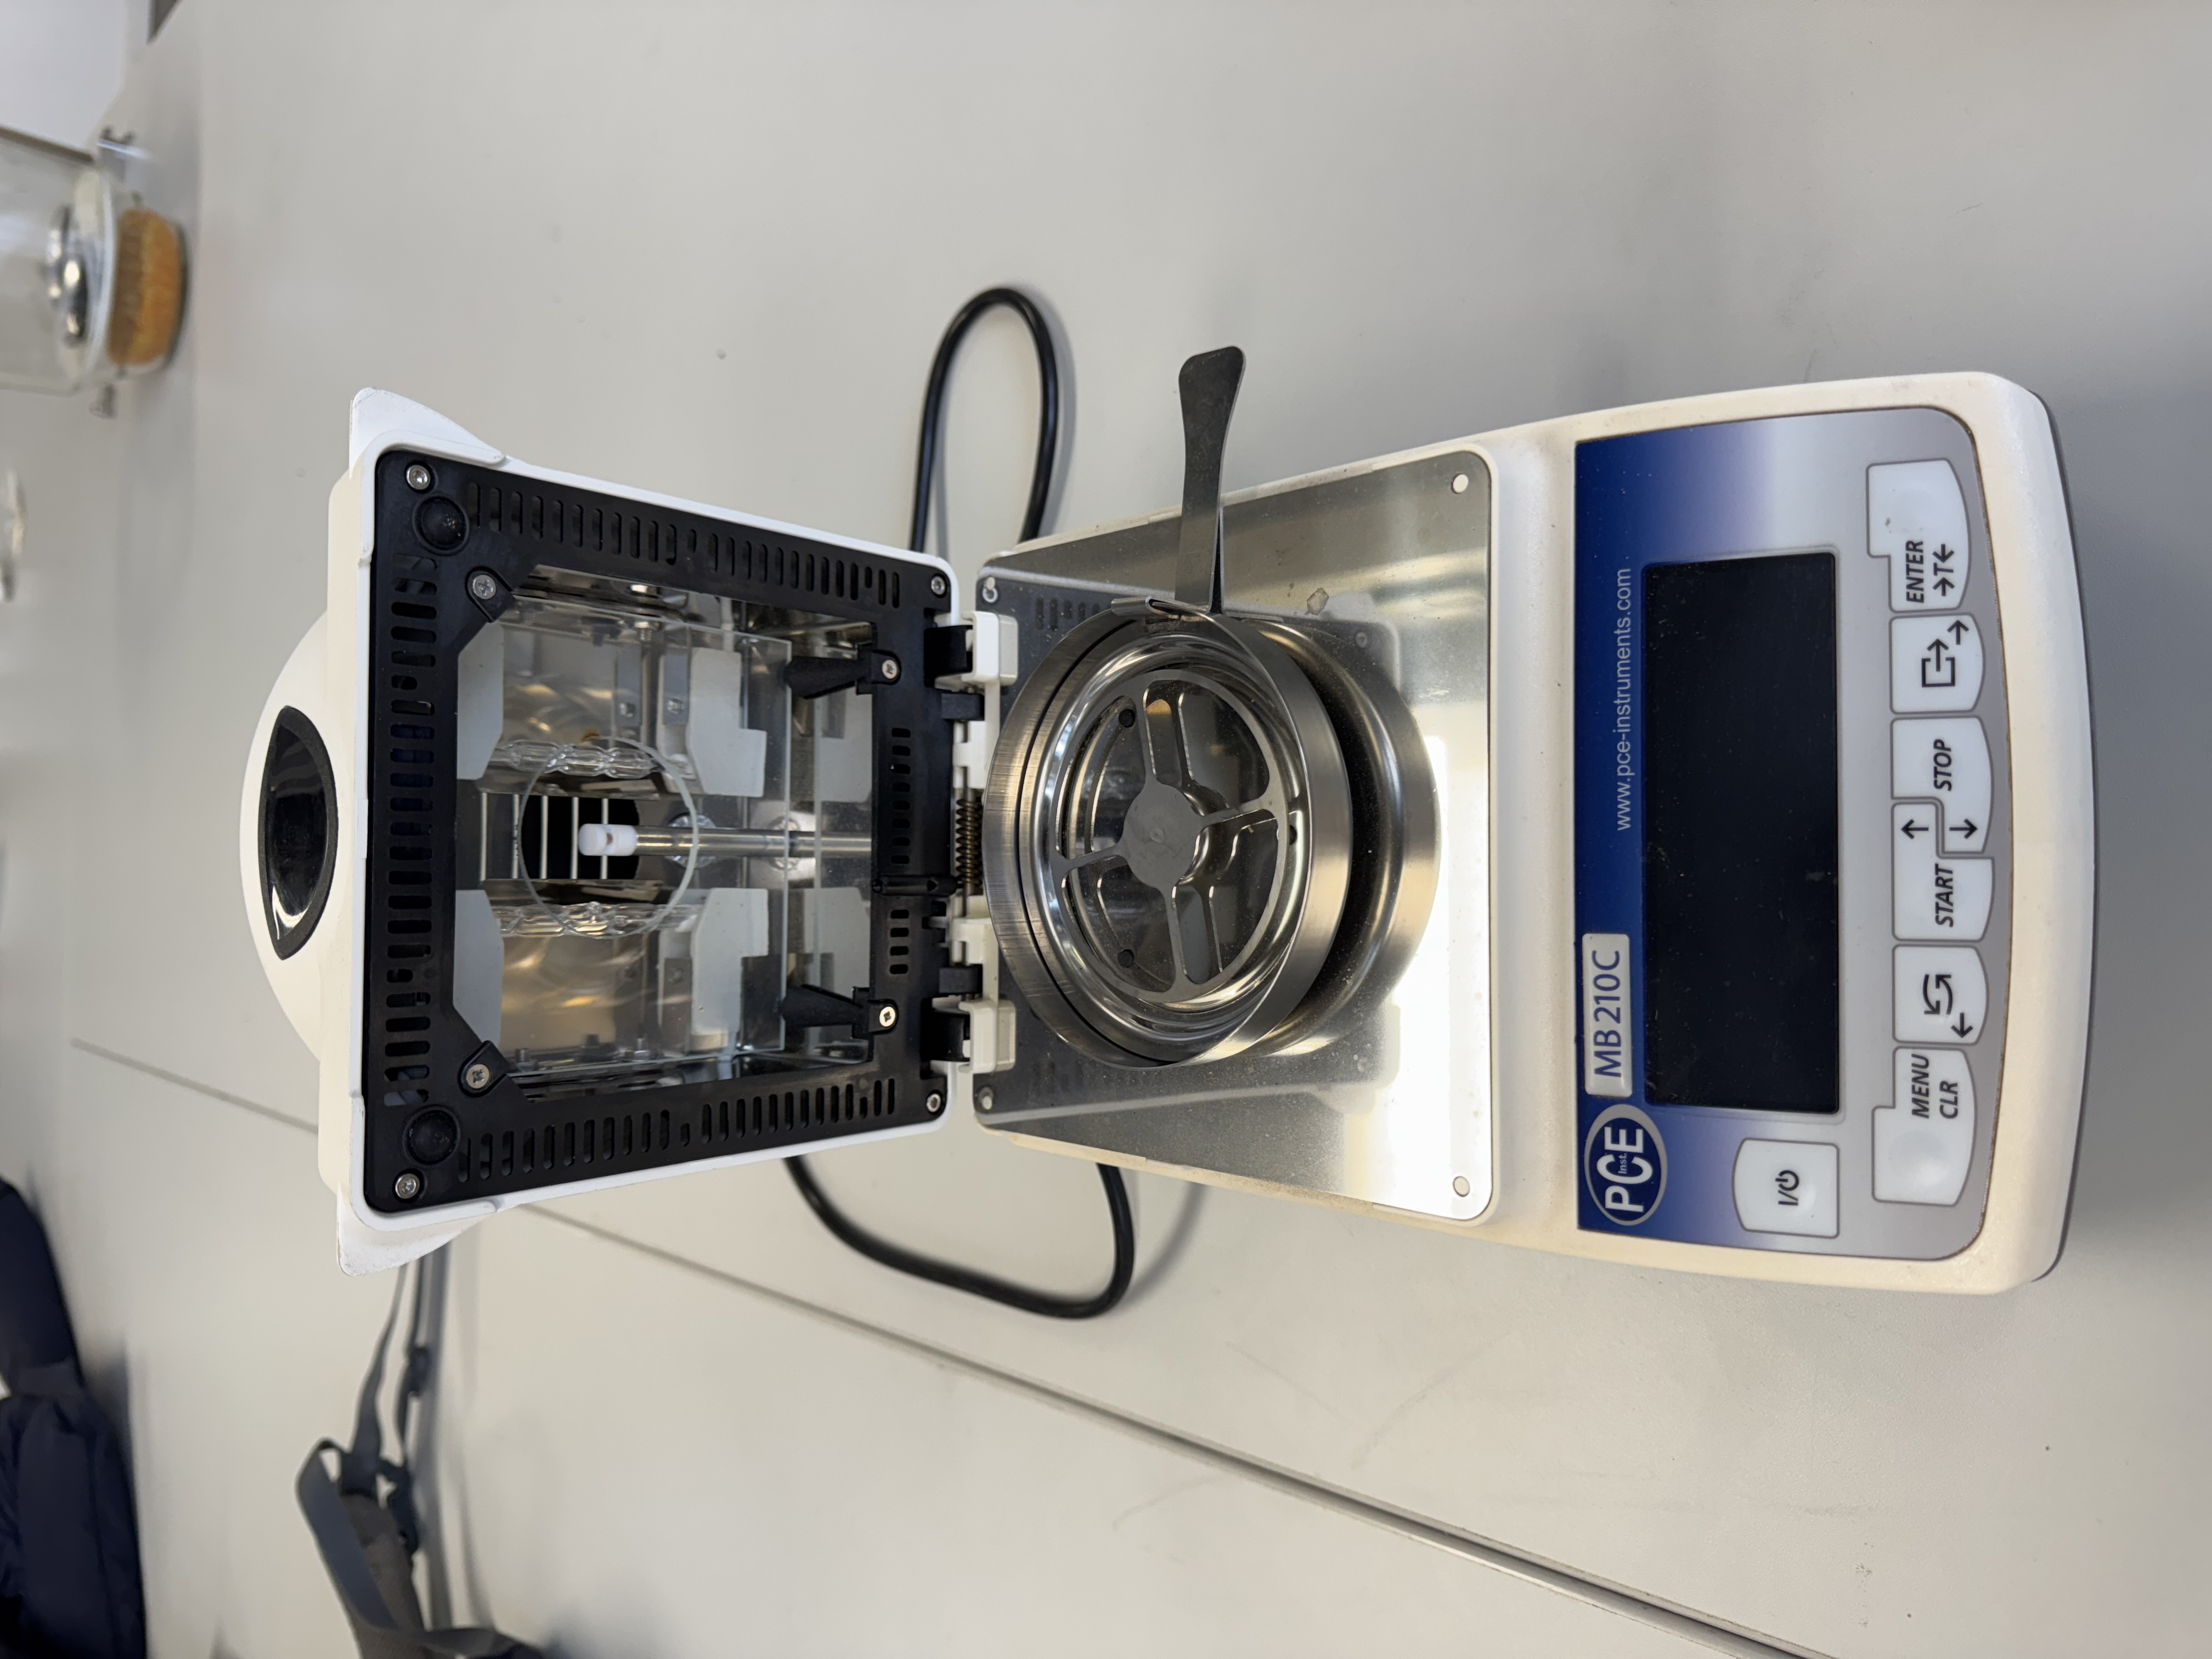
\includegraphics[
        angle=-90,
        origin=c,
        height=0.40\textheight,
        keepaspectratio
    ]{Abbildungen/moisture analyzer.jpeg}
    \caption{Halogen moisture analyzer PCE-MB 210C}
    \label{fig:moisture_analyzer}
\end{figure}

\vspace{0.3em}

For each measurement, approximately 1.0 g of dried biochar was placed in the crucible and then inserted into the bomb. The bomb was sealed and pressurized with pure oxygen to ensure complete combustion. Combustion was initiated electrically via an ignition wire in contact with a thread, which was also in contact with and buried within the biochar. The temperature rise of the surrounding water bath was recorded by the instrument, and the gross calorific value $q_{V,gr}$ was calculated automatically by the device according to Equation \ref{equ: qvgr} in \S~\ref{subsubsec:HHV}.

\vspace{0.3em}

Each biochar was measured in triplicate (n=3). Mean values and standard deviations are reported in Chapter \ref{Section:result}. 


\subsubsection{Ash Content Determination}
\label{subsubsec:methods-ash}
The ash content was not determined in a separate ashing campaign. It was taken from the
calorific value determination runs described in \S~\ref{subsubsec:methods-calorimetry}, each of which leaves a
mineral residue in the crucible once the organic fraction has burned off.

\vspace{0.3em}

The empty crucible was tared on the analytical balance, and the dried biochar was weighed into it, giving the initial mass $m_0$. After the bomb had been depressurized and opened, the crucible was weighed again with the residue still inside. The residue mass $m_{\mathrm{ash}}$ is the difference between the two readings, and the ash content follows as

\begin{equation}
\mathrm{Ash} = \frac{m_{\mathrm{ash}}}{m_0} \times 100\,\%
\label{eq:ash-content}
\end{equation}

Since every calorimetric run yields one ash value, the triplicate measurement gives three ash
values per material. Means and standard deviations are reported alongside the calorific values
in Chapter~\ref{Section:result}, and the individual weighings are listed in
Table~\ref{tab:calorific-full}. Ash was determined this way for the raw French digestate and for
the three pristine biochars. The activated and sulfur-loaded chars were not measured, which is
why no ash-free basis and no oxygen-by-difference can be given for them
(\S~\ref{subsubsec:methods-chns}).

\vspace{0.3em}

This procedure does not constitute a standard ash determination. According to DIN EN ISO 18122 for solid biofuels and ASTM E1755 for biomass, ash content is determined by heating the sample in a muffle furnace in air at approximately 550~$^\circ$C until a constant mass is reached \cite{96,97}. In contrast, the residue measured here resulted from a short combustion step rather than from complete ashing under standardized conditions.

This is not a standard ash determination. Accordiing to DIN EN ISO 18122 for
solid biofuels and ASTM E1755 for biomass, both ash the sample in a muffle furnace in air at
550\,$^{\circ}$C and hold it until the mass is constant \parencite{iso18122_2022, astm_e1755_2020}. The residue weighed here comes instead from a short combustion in pressurized pure oxygen, at no defined holding temperature and no defined holding time. Carbonates and other thermally labile minerals may therefore decompose to a different extent than they would in a furnace, and traces of unburned carbon can remain in the crucible. The values reported in this work are combustion residues, defined by the calorimetric procedure itself, and they are not strictly comparable with ash contents measured according to the standards above. The procedure was used because it costs no additional sample material and requires no separate furnace run, and because the ash values enter this work as a correction factor for converting results to an ash-free basis \parencite{iso16993_2016} rather than as a fuel specification reported in its own right.

\subsubsection{BET Analysis}

The BET analysis was outsourced to the Chair for Energy Process Engineering and Conversion Technologies for Renewable Energies (Fachgebiet Energieverfahrenstechnik und Umwandlungstechniken regenerativer Energien, EVUR), Institute of Energy Technology, Faculty III -- Process Sciences, Technische Universität Berlin (TU Berlin), as the corresponding equipment and instrumentation were not available at HTW Berlin. The analysis used a BET analyzer with the model Sync220A and a static volumetric method. This analysis used nitrogen as the adsorbate, and the measurement was done at 77.35 K. The analysis required approximately 2 hours. Only the pristine and activated, sulfur-enriched French biochars were subjected to BET analysis due to budgetary reasons and lower mass loss during the activation.

\vspace{0.3em}

The results of the analysis include the specific surface area (SSA), the total pore volume, and the mean pore diameter. Since the results are based on two measurements conducted under the same conditions, the final values for the SSA and the total pore volume are reported as averages. Therefore, the mean pore diameter determined by BET analysis is not used and is subsequently calculated from the average value of SSA and total pore volume as follows:

\begin{equation}
\text{Mean pore diameter} = \frac{4 *\text{Total pore volume}}{\text{Specific surface area}} =\frac{4V_p}{A}
\label{Equation mean pore}
\end{equation}

%\vspace{0.3em}

\subsubsection{CHNS Elemental Analysis}
\label{subsubsec:methods-chns}
The elemental analysis was also outsourced to EVUR. The mass fractions of carbon (C), hydrogen (H), nitrogen (N), and sulfur (S) in the pristine biochar, as well as in the activated, sulfur-loaded biochars were determined by combustion-based elemental analysis. The analysis consisted of four individual measurements, which were then calculated and presented as an arithmetic mean. These individual measurements were not released by the laboratory of TU Berlin, which means no scatter can be shown.

\vspace{0.3em}

Since the analysis only determined the CHNS elements, the fraction of oxygen was not included in the measurement. However, assuming that the sum of C, H, N, S, O, and ash accounts for the whole biochar composition, the fraction of oxygen can presumably be calculated as follows:  

\begin{equation}
O = 100\% - (C + H + N + S + \mathrm{ash})
\label{eq:O_fraction}
\end{equation}



